\chapter{Boosted Decision Trees}
\label{chap:Appendix:BDT}


% igual puedo sacarme alguna idea de aquí: https://cds.cern.ch/record/2836731?ln=en
% sacar alguna idea de aquí: https://arxiv.org/pdf/2206.09645.pdf

%\section{Intro}
A boosted decision tree, typically referred just by its acronym BDT, is a supervised\footnote{Supervised learning means that the 
data used in the training is labeled.} machine learning (ML) technique used for classification. The analysis presented in this thesis 
uses several BDTs. Both the light lepton origin assignment (Section \ref{sec:ChaptH:Sig:LepAsign}) and the signal to background 
separation (Section \ref{sec:ChaptH:EventSelection:BDT}) are based on a BDT. This tool is applied in more scenarios within 
within ATLAS. In the \btag, for instance, a BDT is trained to discriminate \bjets from light-jets \cite{Connelly:2017wlp}. 



%Paragraphs of section intro
%\begin{itemize}
%	\item What is Machine Learning and an MVA method
%	\item what is a BDT
	% source: https://hastie.su.domains/Papers/ESLII.pdf    
		% Chapter Tree-Based Methods
		% Chapter 10: Boosting and Additive Trees
%	\item Uses of the BDT in this thesis: Two different libraries for TMVA ROOT and XGBoost. For XGBoost we have
%	 to convert the data to ¿pandas?¿numpy?
%	\item BDT in comparison to NN	
%\end{itemize}

\section{How does a BDT work?}
A BDT is an ensamble of decision trees. Each decision tree is a map of possible results of related decisions. 
A decision tree takes a set of input features and splits input data recursively based on those features. 
This results in a tree structure that resembles that of a flow charts with a decision or split at each node.
The last level of the trees are the so called leaves and each represents a class.
An example of a tree can be seen on Figure \ref{fig:Appendix:BDT:TreeExample}, where an event is classified in one of the two 
categories following a set of yes-no questions. In this work the BDTs employed are binary, i.e. separates into two categories, 
but multiclassifier BDTs could be used as well\footnote{For the signal to background discrimination, multiclassifer BDTs were
tested but the result was not satisfactory.}.


\begin{figure}
\centering
  \centering
  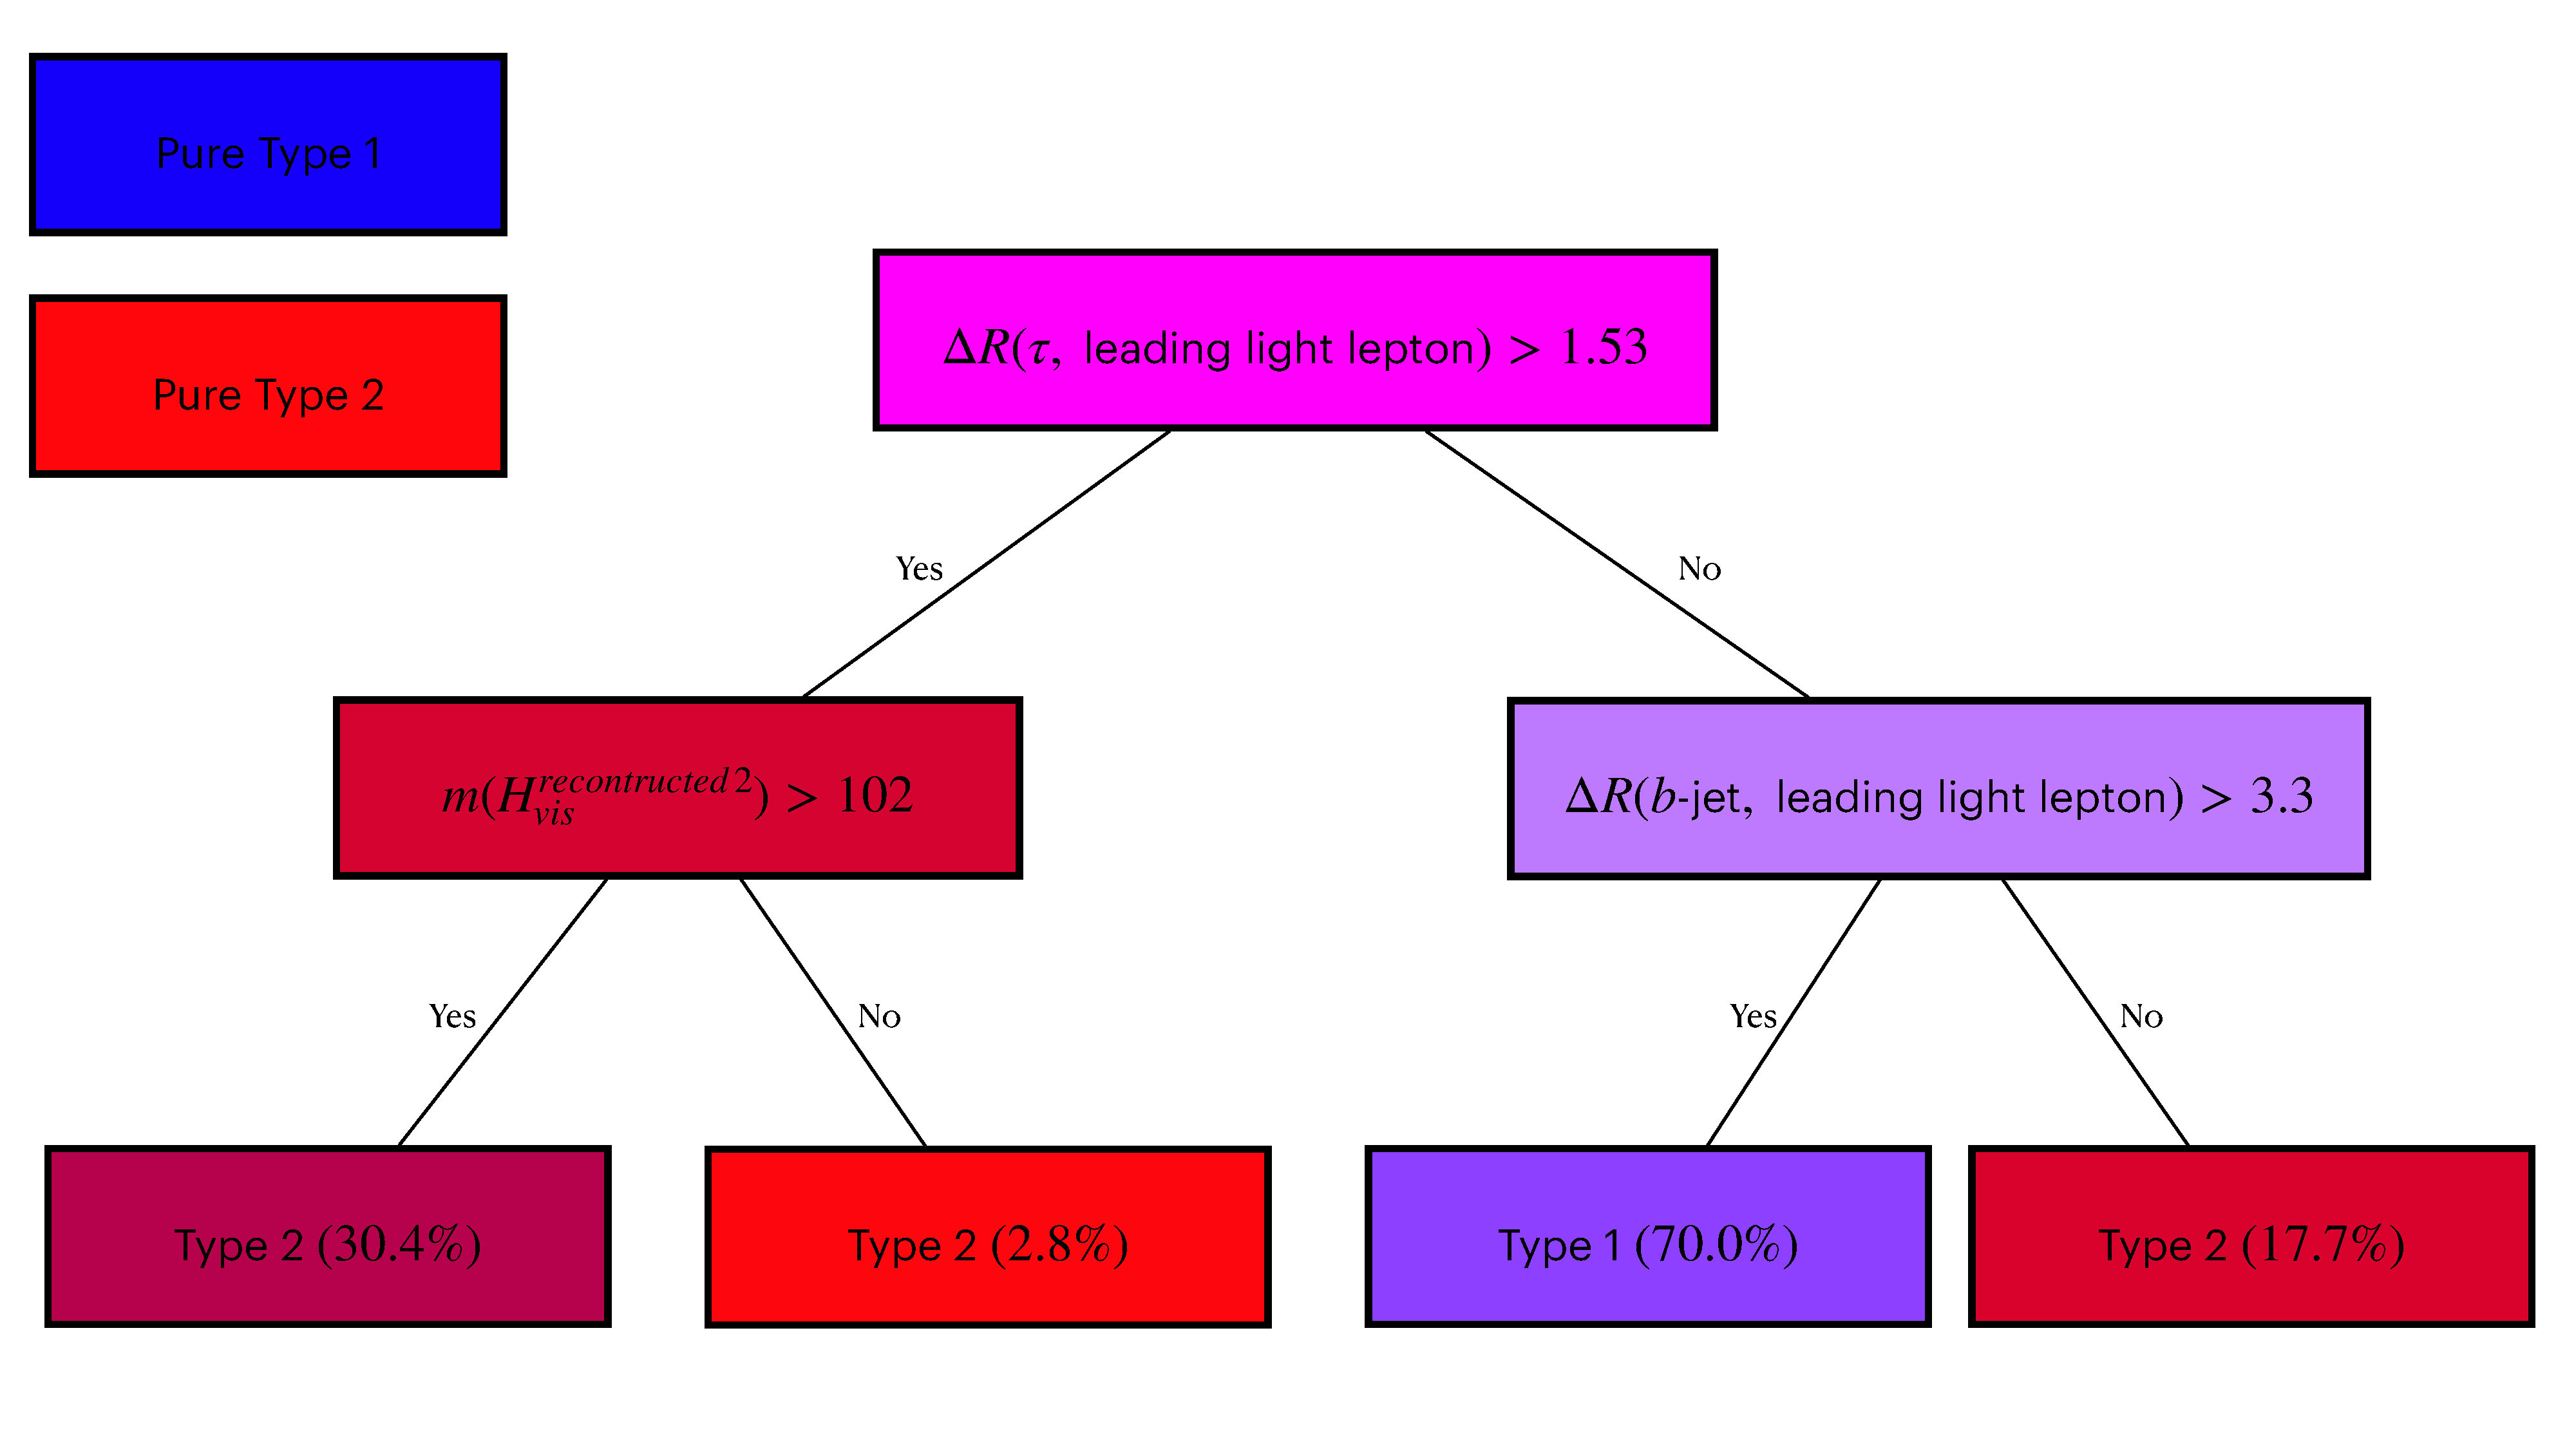
\includegraphics[width=.9\linewidth]{Appendices/BDT/BDT_Assignment_singleTree}
\caption{Example of a decision tree with three nodes. This particular example corresponds to one of the trees in the BDT for the 
light lepton origin assignment (see Section \ref{sec:ChaptH:Sig:LepAsign}). The color of the boxes represents the purity on Type 1 or Type 2 events that arrive to each node. Repeated left/right (yes/no) decisions are taken on one single variable at
a time until the classification takes place.}
\label{fig:Appendix:BDT:TreeExample}
\end{figure}

Boosting is a technique for turning numerous weak classifiers (trees in this case) into a powerful one. 
Each tree is created iteratively depending on the prior ones. The output of each tree, $h_{t}(\bm{x})$, is given a weight, $w_{t}$,
relative to its accuracy. The ensamble output is the weighted sum
\begin{equation*}
	\hat{y} (\bm{x}) = \sum_{t} w_{t}h_{t}(\bm{x})
\end{equation*}
where $t$ run over the trees. The goal of the boosting is to minimise a regularised objective function
\begin{equation}
\label{eq:Appendix:BDT:ObjectiveFunction}
	L (x) = \sum_{i} l(\hat{y}_{i}, y_{i})+ \sum_{t}\Omega(f_{t}) \,
\end{equation}

where $l(\hat{y}_{i}, y_{i})=l(f(\bm{x}_{i}|\theta), y_{i})$ is a differentiable convex
 loss function (the distance between the truth and the prediction of the i$^{th}$ sample) and
$\Omega(f_{t})$ is the regularisation function (penalises the complexity of the $t^{th}$ tree, $f_t$).
The $\theta$ in $f(\bm{x}_{i}|\theta)$ are the model parameters for a BDT these would be the weights
and biases. The $\bm{x}_i$ are values fo the input 
variables for the i$^{th}$ sample and $y_{i}$ the target variable real value. 

The $\Omega(f_{t})$ term helps to smooth the final learnt weights to avoid
over-fitting. %There are several types of loss functions such as Huber, Least Squares, Absolute Deviation, etc


The tree ensemble model in Eq. \ref{eq:Appendix:BDT:ObjectiveFunction} cannot be optimised using 
traditional optimisation methods in Euclidean space. 
The model is trained instead in an additive way so that the objective function to minimise is:
\begin{equation}
\label{eq:Appendix:BDT:ObjectiveFunction_alternative}
	L^{(t)} =  \sum_{i}^n l(y_i, \hat{y}_i^{(t-1)} + f_t(\bm{x}_i)) + \Omega (f_t) \,.
\end{equation}

There are several types of boosting for BDTs. Some of the most common are AdaBoost, Gradient Boosting and XGBoost. 
The later, which stands for ``eXtreme Gradient Boosting'', is the used in this work and its details can be found in reference \cite{Chen_2016}.
Boosting can significantly improve performance compared to that of a single tree and stabilise 
the response of the decision trees to fluctuations in the training sample.


\pablo{Para evaluar la log loss usamos la función log\_loss de skalearn: https://scikit-learn.org/stable/modules/generated/sklearn.metrics.log_loss.html}


\subsection{Training}
For a ML algorithm, to train means to learn or determine good values for all the weights within that model. 
To do so, the algorithm takes the labelled data and fits the model. For instance, for the signal discrimination,
the ML model takes the MC samples, where all the events are labeled either as signal or background events. 
A renormalisation can take place if needed. 
With the data, the model also needs 
a set of variables that have some power to discriminate between our categories.  A condition on one discriminant variable
is set on each node of the BDT to split the phase space into two parts.
The aim of the training is to find the optimal cut in each node so that after it
the separation between the categories is maximised, in our example one category is enriched in background and the other in signal.  
This is done in a loop over all discriminating variables and trying to test as many as possible values for each cut 
(the default in TMVA is trying 20 values for each variable). The best splitting in defined on the basis of the splitting index,
which works as a mesure of inequality becase we want to measure the inequality between the two categories in each split node. 
A low splitting index value means a high inequality between the classes, i.e. high purity.
%There ara several splitting indices like the gini index, the cross-entropy, missclassification error, statistical significance and others
%they all hace similar performance.
The best cut is defined as the one the one that yields the highest splitting index difference between the parent node
and the two children node (each weighted by the total number of events in the corresponding block). 
Then it is possible keep splitting blocks until a stoping requirement is satisfied. 
%A single tree is a very weak classifier because it is very sensitive to statistical fluctuations in the training MC sample. 
%To increase the sensitivity power of the tree, a solution is create many of them and take an average output.   



\paragraph{Internal reweight of events in training sample}\mbox{}\\
Sometimes, MC generators may provide event weights which may turn out to be extremely small or very high. To avoid
artefacts, TMVA can renormalise the signal and background training weights internally so that their respective sums of 
effective (weighted) events are equal. By doing this, the performance of the BDT can be improved since some 
classifiers are sensitive to the relative amount of each category (Type1/Type2 or signal/background) in the training data.
While for the lepton assignment this renomalisation does not play an important role (the amount of Type1 and Type2 
signal events is similar), for the \tHq signal discrimination the signal sample in the training test has to be reweighted.

\subsubsection{Loss function}
Sometimes called error function, the loss function is used to define what is a good prediction and what is not by
assessing how far an estimated value is from its true value for a particular model iteration and penalising errors in
the prediction.
%In other words,
%it evaluates how far a certain model iteration is from the actual values.
Therefore, it is crucial to any supervised ML model.
Depending on whether the model is for a regression or for classification, 
the way $ l(y_{n}, f(\bm{x}_{n}|\theta))$ is defined may vary and, for the analysis,
only binary classification BDTs have been used. 

Classification problems include foreseeing a discrete class output. 
It entails categorising the dataset into distinct categories based on 
various factors (variables) so that when new and unseen data appears 
it can be classified as well. 

\paragraph{XGBoost loss functions}\mbox{}\\ %source: https://machinelearningmastery.com/xgboost-loss-functions/
The loss function that have been used for predicting probabilities for the binary classification 
in the signal selection is “binary:logistic” but there are other available options such as
 “binary:logitraw” and “binary:hinge”. Some tests were carried using a multiclass BDT, for those
 the “multi:softprob“ loss function was used. 
 
When using the binary logistic loss function of XGBoost, the
$l$ in Eq \ref{eq:Appendix:BDT:ObjectiveFunction_alternative} 
is the logarithmic likelihood of the Bernoulli distribution and it %maybe comment this line
takes the form
\begin{equation}
\label{eq:Appendix:BDT:binaryLogistic_A}
	l = y_i \log[\text{logistic}(\hat{y}_i^{(t-1)} + f_t(\bm{x}_i))] + (1-y_i)\log[1-\text{logistic}(\hat{y}_i^{(t-1)} + f_t(\bm{x}_i))] \,
\end{equation}
where $\text{logistic}(\hat{y}_i^{(t-1)} + f_t(\bm{x}_i))$ is the probability.  In an algebraically equivalent
manner, it can be written as:
\begin{equation}
\label{eq:Appendix:BDT:binaryLogistic_B}
	l = y_i [\hat{y}_i^{t-1} + f_t(\bm{x}_i)) - \log(1 + \exp (\hat{y}_i^{t-1} + f_t(\bm{x}_i))]
\end{equation}


Other loss functions
\begin{itemize}
	\item \textbf{binary:logistic}: Logistic regression for binary classification, output probability
	\item \textbf{binary:logitraw}: Logistic regression for binary classification, output score before logistic transformation
	\item \textbf{binary:hinge}: Hinge loss for binary classification. This makes predictions of 0 or 1, rather than producing probabilities.
	\begin{equation}
		l(f(x_i|\theta), y_i) = \max(0, 1-f(x_i|\theta)y_i)
	\end{equation} % more about hinge https://www.section.io/engineering-education/understanding-loss-functions-in-machine-learning/#loss-functions-for-classification
	
\end{itemize}


\subsubsection{Overtraining}
\label{chap:Appendix:BDT:Overtraining} 
% Source https://root.cern.ch/download/doc/tmva/TMVAUsersGuide.pdf
% From page 31 - Cross Validation

Let's consider a ML model $f(\bm{x}|\theta)$, where $x$ are the data points used as input and $\theta$
the tuneable parameters of the model. The function $f(\bm{x}|\theta)$ outputs the prediction of the model.
The parameters $\theta$ of the model are tuned during the training process using a training set 
($\mathcal{T}$). The true output ($y$) of the elements in $\mathcal{T}$.
When successful, the training finds the $\theta$ that performs as good as possible on new, 
unseen, data.

For a given $f(\bm{x}|\theta)$ model, the training error, $\text{err}(\mathcal{T})$, is defined by 
\cite{zimmermann2006statistical}:
\begin{equation}
\label{eq:Appendix:BDT:ErrorOfTest}
	\text{err}(\mathcal{T}) = \frac{1}{N_t} \sum_{n=1}^{N_t} l(y_{n}, f(\bm{x}_{n}|\theta)) 
\end{equation}
where $N_t$ is the number of events used for the training and $l$ the chosen loss function and
$\bm{x}_n$ and $y_n$ the points in the training set. So, the error function measures the model’s 
error on a group of objects, whereas the loss function deals with a single data instance.

The $\text{err}(\mathcal{T})$ is a poor estimator of the model's performance on new
 data. It usually decreases as the number of training cycles increases, and it can begin 
 to adapt to noise in the training data. When this happens the training error continues to 
 decrease but the error on the data outside of the training set starts increasing, jeopardising
 the general performance of the model. This effect is the so called overfitting or overtraining.
 

Overtraining occurs when a ML model can accurately predict training examples but is 
unable to generalise\footnote{By generalise is meant that the model recognises only 
those characteristics of the data that are general enough to also apply to some unseen data.}
 to new data.  When overtraining takes place, the ML model has learnt
the details of the training data to an extent in which these knowledge do not reflect the 
behaviour of the test sample.  This results in poor field performance. 

Figure \ref{fig:Appendix:BDT:Overtrain} shows how an overtrained BDT evolves. 
In Figure \ref{fig:Appendix:BDT:Overtrain:AUC} can be seen that as the training of the
BDT continues, the ability of the model to classify the events in $\mathcal{T}$ (blue)
improves while for the data in the test sample (orange) it doesn't. This means that
the model is not generalising properly. 
With the plot of the loss function (Figure \ref{fig:Appendix:BDT:Overtrain:LogLoss})
can be seen how the error of the test data slightly increases while for the training
samples is strongly reduced. 


\begin{figure}
\centering
\begin{subfigure}{.475\textwidth}
  \centering
  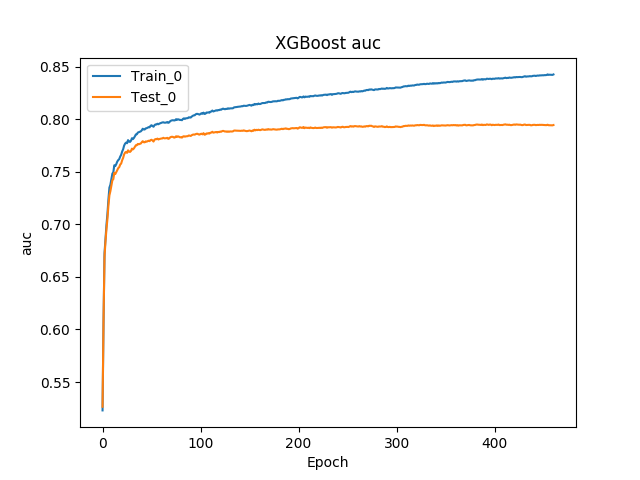
\includegraphics[width=.9\linewidth]{Appendices/BDT/OvertrainingExamples_AUC_SR_tHq_OS}
  \caption{Area under the ROC curve.}
  \label{fig:Appendix:BDT:Overtrain:AUC}
\end{subfigure}%
\begin{subfigure}{.475\textwidth}
  \centering
  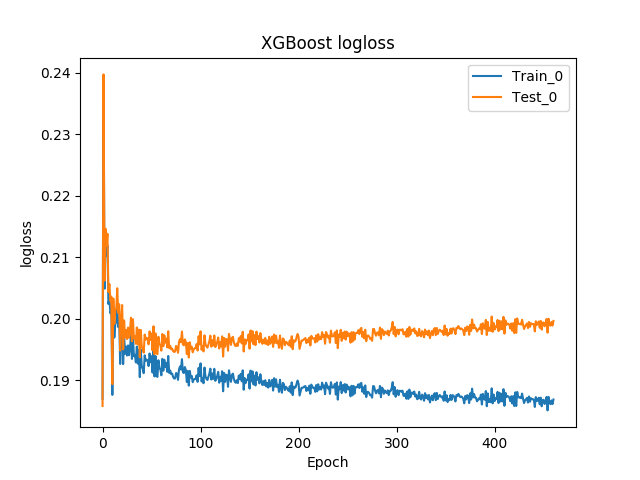
\includegraphics[width=.9\linewidth]{Appendices/BDT/OvertrainingExamples_LogLoss_SR_tHq_OS}
  \caption{Logarithm of the loss function.}
  \label{fig:Appendix:BDT:Overtrain:LogLoss}
\end{subfigure}
\caption{Example of the evolution of the BDT metrics when overtraining occurs. The x-axis shows the training iteration. Observe how the curves for the train and test samples diverge as the training epochs advance.}
\label{fig:Appendix:BDT:Overtrain}
\end{figure}


When tested on the training sample, overtraining results in an apparent improvement 
in classification or regression performance over the objectively achievable one, but an 
effective performance loss when measured on an independent test sample (even though, 
there is a risk that it can still happen even if we use separate test data).
Until deployed to real unseen data, there is a danger that
overtraining will go unnoticed. This makes of overtraining one of the greatest dangers in ML.
Other names for this phenomenon are overfitting and type III error.

Usually, this is a result of too little data or data that is too homogenous.
Overtraining arises when there are too few degrees of freedom, because too many model parameters of an algorithm
were adjusted to too few data points.  Not all MVA methods are equally sensible to overtraining.  While Fisher 
discriminant hardly suffers from it, BDTs usually suffer from at least partial overtraining, owing to their large number of 
nodes. Nevertheless, for the BDTs some countermeasures can be applied to preserve the ability to generalise:

\begin{itemize}
	\item Never test the model on the data used for the training.
	\item The number of nodes in boosted decision trees can be reduced by removing 
		insignificant ones (``tree pruning''). There are to types, pre-pruning and post-pruning
		\begin{itemize}
			\item Pre-pruning: Refers to the early stopping of the growth of the decision tree
				% In XGBoost "max_depth"
			\item Post-pruning: Allows the decision tree model to grow to its full depth, then removes 
				the tree branches to prevent the model from overfitting
		\end{itemize}
	\item Cross validation is a powerful technique to use all the data for training at the same 
		time that all the data for testing is employed while avoiding overfitting. This method is
		based in cleverly iterating the test and training split around and it is described in 
		Section \ref{chap:Appendix:BDT:kfold}.
\end{itemize}
%https://indico.cern.ch/event/294651/contributions/671918/attachments/552028/760654/ESIPAP_MVA130129-BDT2.pdf






\subsection{Evaluation / Validation}
%The test set should ideally only be used only once to evaluate a model's performance. 
%When a data set is reused, it introduces some bias. Trying out numerous ideas in the 
%early stages of an analysis is a frequent practise to figure out what works and what 
%doesn't. Model selection is the process of choosing the best model from a group of ideas.
%Model selection refers not only to chosen between the types (BDT, Neural Network, k-nearest
%neighbours, SVN, etc) but also about choosing the hyperparameters for a model.




\subsection{Application}

\section{Treatment of negative weights}
\label{chap:Appendix:BDT:NegWeigts}

\subsection{BDT for Lepton origin assignment}
\label{chap:Appendix:BDT:NegWeigts:TMVARoot}
The ROOT.TMVA library offers several possibilities to deal with the negatively weighted events.
These are:
\begin{itemize}
	\item InverseBoostNegWeights: It boosts with inverse boostweight.
		This option is not available for gradient boosting.
	\item IgnoreNegWeightsInTraining: This offers 
	\item Pray: This option allows to use negative weights in the training but might cause 
		problems with small node sizes or with the boosting. It was tested and the model could not
		achieve stability. 
	\item PairNegWeightsGlobal: This option is still experimental. It takes the negatively 
		weighted events and pairs them with the events with positive weights, anihilating both.
		When using this option the gradient BDT was not able to converge.
\end{itemize}
In the BDT for determining the light-lepton origin, the selected treatment is ignoring the negative weights 
in the training. When testing the model, these weights are taken into account.


\section{Cross validation and \textit{k}-folding}
\label{chap:Appendix:BDT:kfold}
Cross validation is a technique consisting in training several ML models on different subsets of the input data
and evaluated on the complementary subset of the data. The goal cross validation is to estimate the
performance of a machine learning model. It can identify overfitting or recognise the failure of the model to
generalise a pattern.

One particular method to do this is the \textit{k}-folding. It consists on splitting the input data into 
$k \in \mathcal{N}$ equally-sized subsets. Each of these is known as fold. With this procedure the ML model is 
trained \textit{k} times. For each train $k-1$ folds are used as training set and the non-used fold is the subset 
of date where the evaluation takes place. All folds are used once as test sample and $k-1$ times in the train 
sample. 

\begin{figure}
\centering
  \centering
  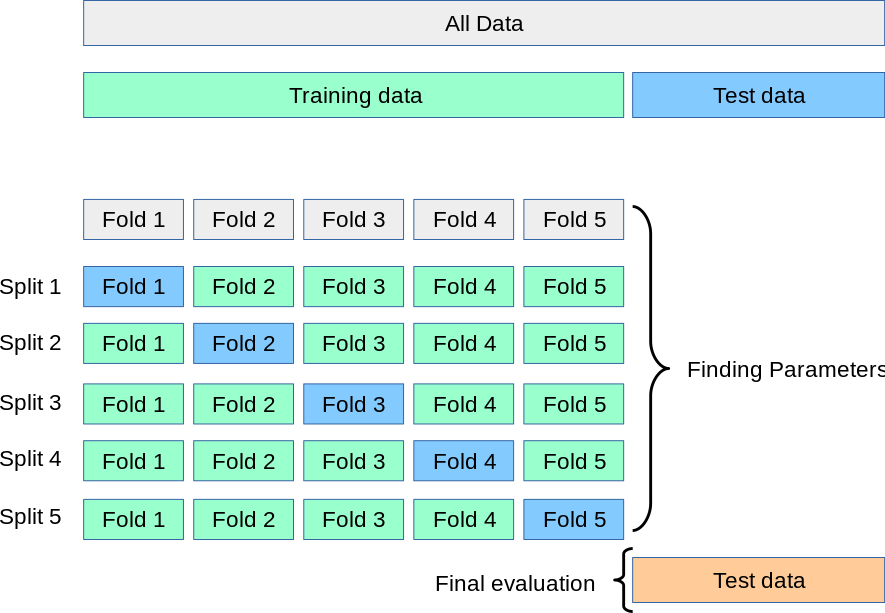
\includegraphics[width=.9\linewidth]{Chapter5_tHq/BDT_generalities/k_folding_cross_validation.png}
\caption{Illustration of \textit{k}-folding cross validation using 5 folds.}
\label{fig:Appendix:BDT:kfold}
\end{figure}

\textit{k}-folding cross validation resample is of particular interest when the data available is limited 
because, by using it, all events are used in the training phase.  It generally results in a less biased 
or less optimistic estimate of the model skill than other methods, such as a simple train/test split.

Note that when the score of the model is applied, each event gets the score that was assigned when
it was used as test event. Not doing this would bias the model.

The expected error for a $f(x|\theta)$ trained using \textit{k}-folding is:
\begin{equation}
\label{eq:Appendix:BDT:ErrorKFold}
	\text{err}(\mathcal{T}) = \frac{1}{k} \sum_{k} \text{err}(\mathcal{T}_{k}) ,
\end{equation}
where $\text{err}(\mathcal{T}_{k})$ is the error as described in Eq. \ref{eq:Appendix:BDT:ErrorOfTest} for each splits test.
As Eq. \ref{eq:Appendix:BDT:ErrorKFold} shows, an increase on the number of folds would imply more
models to average over and, hence, implying an improvement on the confidence of how consistent 
the $f(x|\theta)$ achieves a given level of performance. However, a larger $k$ would also reduce
the statistical strength of each fold.

\pablo{Should I comment that the event number is the variable used to 
split the samples into different folds so that we can later assign the score properly?}
%A problem with \textit{k}-folding is that the estimation
%is not done for the final model, but rather of the average final model.



%%%%%%%%%%%%%%
%   Other considerations   %
%%%%%%%%%%%%%%

%\begin{comment}
\section{Other considerations about BDTs}
\label{chap:Appendix:BDT:Concepts}
\paragraph{Binary splits}\mbox{}\\
Rather than splitting into two groups at each node, one could consider
several splits at each stage. Although this has its benefits, it is not a wise 
general course of action. Multiway splits cause the data to fragment too quickly, 
leaving the next level below with insufficient data. At the end, binary splits are 
favoured because they can also be used to create multiclass divides.


% Inestability
\paragraph{Instability of trees}\mbox{}\\
The large variance of trees is one of their main issues. A little modification in the 
data can frequently lead to very different results. This is mainly caused by the
hierarchical structure of the trees, which causes errors in the top split to cascade 
down to all splits below it. By attempting to employ a more stable split criterion, 
this can be somewhat mitigated, but the fundamental instability remains. It is the 
cost of using the data to infer a straightforward, tree-based structure. 

% ROC
\paragraph{Receiver operating characteristic curve}\mbox{}\\
The receiver operating characteristic curve (ROC) is graphical plot used
that is used to illustrate the ability of a binary classifier. It assesses the 
tradeoff between true positive (TP) and false negative (FP) rates as the parameters of the classification vary.
This is depicted in Figure \ref{fig:Appendix:BDT:ROC_AUC:ROC}. 
\begin{itemize}
	\item \textbf{True positive rate}: Also known as sensitivity. 
	It is the possibility of a positive test conditioned on truly being positive. For instance, it's the probability
	for the BDT in Section \ref{sec:ChaptH:EventSelection:BDT} to identify a \tHq event as such. 
	\item \textbf{False positivity rate}: It can be calculated as 1 - sensitivity. 
	It refers to the possibility of a negative test given that it's truly positive. In the Section \ref{sec:ChaptH:EventSelection:BDT}
	BDT scenario it would be the ability to classify a background event as if it was \tHq signal event.  
\end{itemize}

The area under the curve (AUC) is a commonly used quantitative summary, it measures the
bidimensional area under the ROC from (0,0) to (1,1) as Figure \ref{fig:Appendix:BDT:ROC_AUC:AUC} shows.
The use of the AUC is convenient for several two reasons. Firstly, it is invariant with the scale because it does
not measure absolute values but rates. Secondly, it is invariant with respect to the classification threshold and,
hence, it evaluates quality of the classification model.

\begin{figure}
\begin{subfigure}[h]{0.45\linewidth}
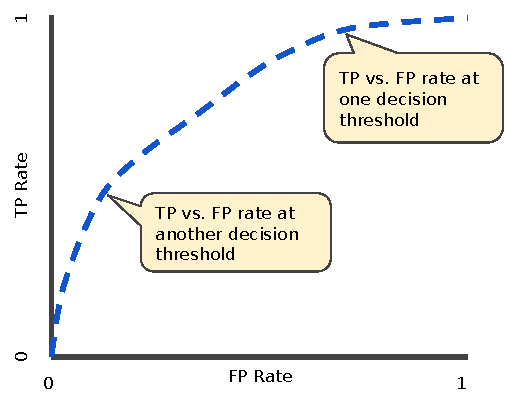
\includegraphics[width=\linewidth]{Appendices/BDT/ROC_AUC_B}
\caption{Typical ROC curve. It shows that as the classification threshold decreases, more events are classified as positive, 
causing both the FP and FN rates to increase.}
\label{fig:Appendix:BDT:ROC_AUC:ROC}
\end{subfigure}
\hfill
\begin{subfigure}[h]{0.45\linewidth}
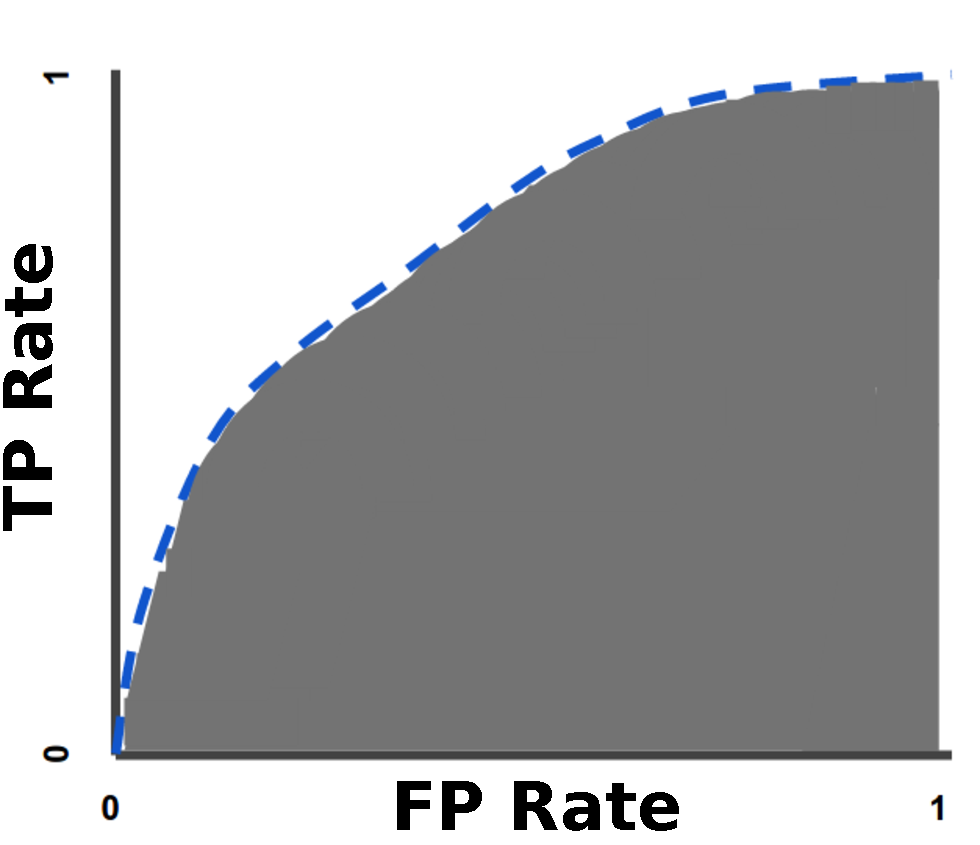
\includegraphics[width=\linewidth]{Appendices/BDT/ROC_AUC_A}
\caption{The AUC varies from 0 to 1. While 0.0 corresponds to a model that always fails, a 1.0 
means that the model is right a 100\% of times.}
\label{fig:Appendix:BDT:ROC_AUC:AUC}
\end{subfigure}%
\caption{The ROC presentes the TP vs the FN rate. The ROC analysis is related
to cost/benefit interpretation of decision making. }
\label{fig:Appendix:BDT:ROC_AUC}
\end{figure}

\pablo{For the meaning of the different AUC values check the reference: \url{https://www.jto.org/article/S1556-0864(15)30604-3/fulltext} \\ 
A perfect predictor gives an AUC-ROC score of 1, a predictor which makes random 
guesses has an AUC-ROC score of 0.5.}

% precision-Recall
\paragraph{Precision-Recall curves}\mbox{}\\
While the ROC shows the summarises the trade-off between 
the true positive rate and false positive rate for a predictive 
for different probability thresholds, there is other plot that helps
with the diagnosis of the binary classification models; the Precision-Recall curves.
These summarise the equilibrium between the true positive rate and 
the positive predictive value for a predictive model using different probability thresholds.

Typically, the use of ROC and precession-recall curves is such that the first type is used
when there are roughly equal numbers of observations for each class and
the second should be used when there is a moderate to large class imbalance.

\begin{figure}
\centering
  \centering
  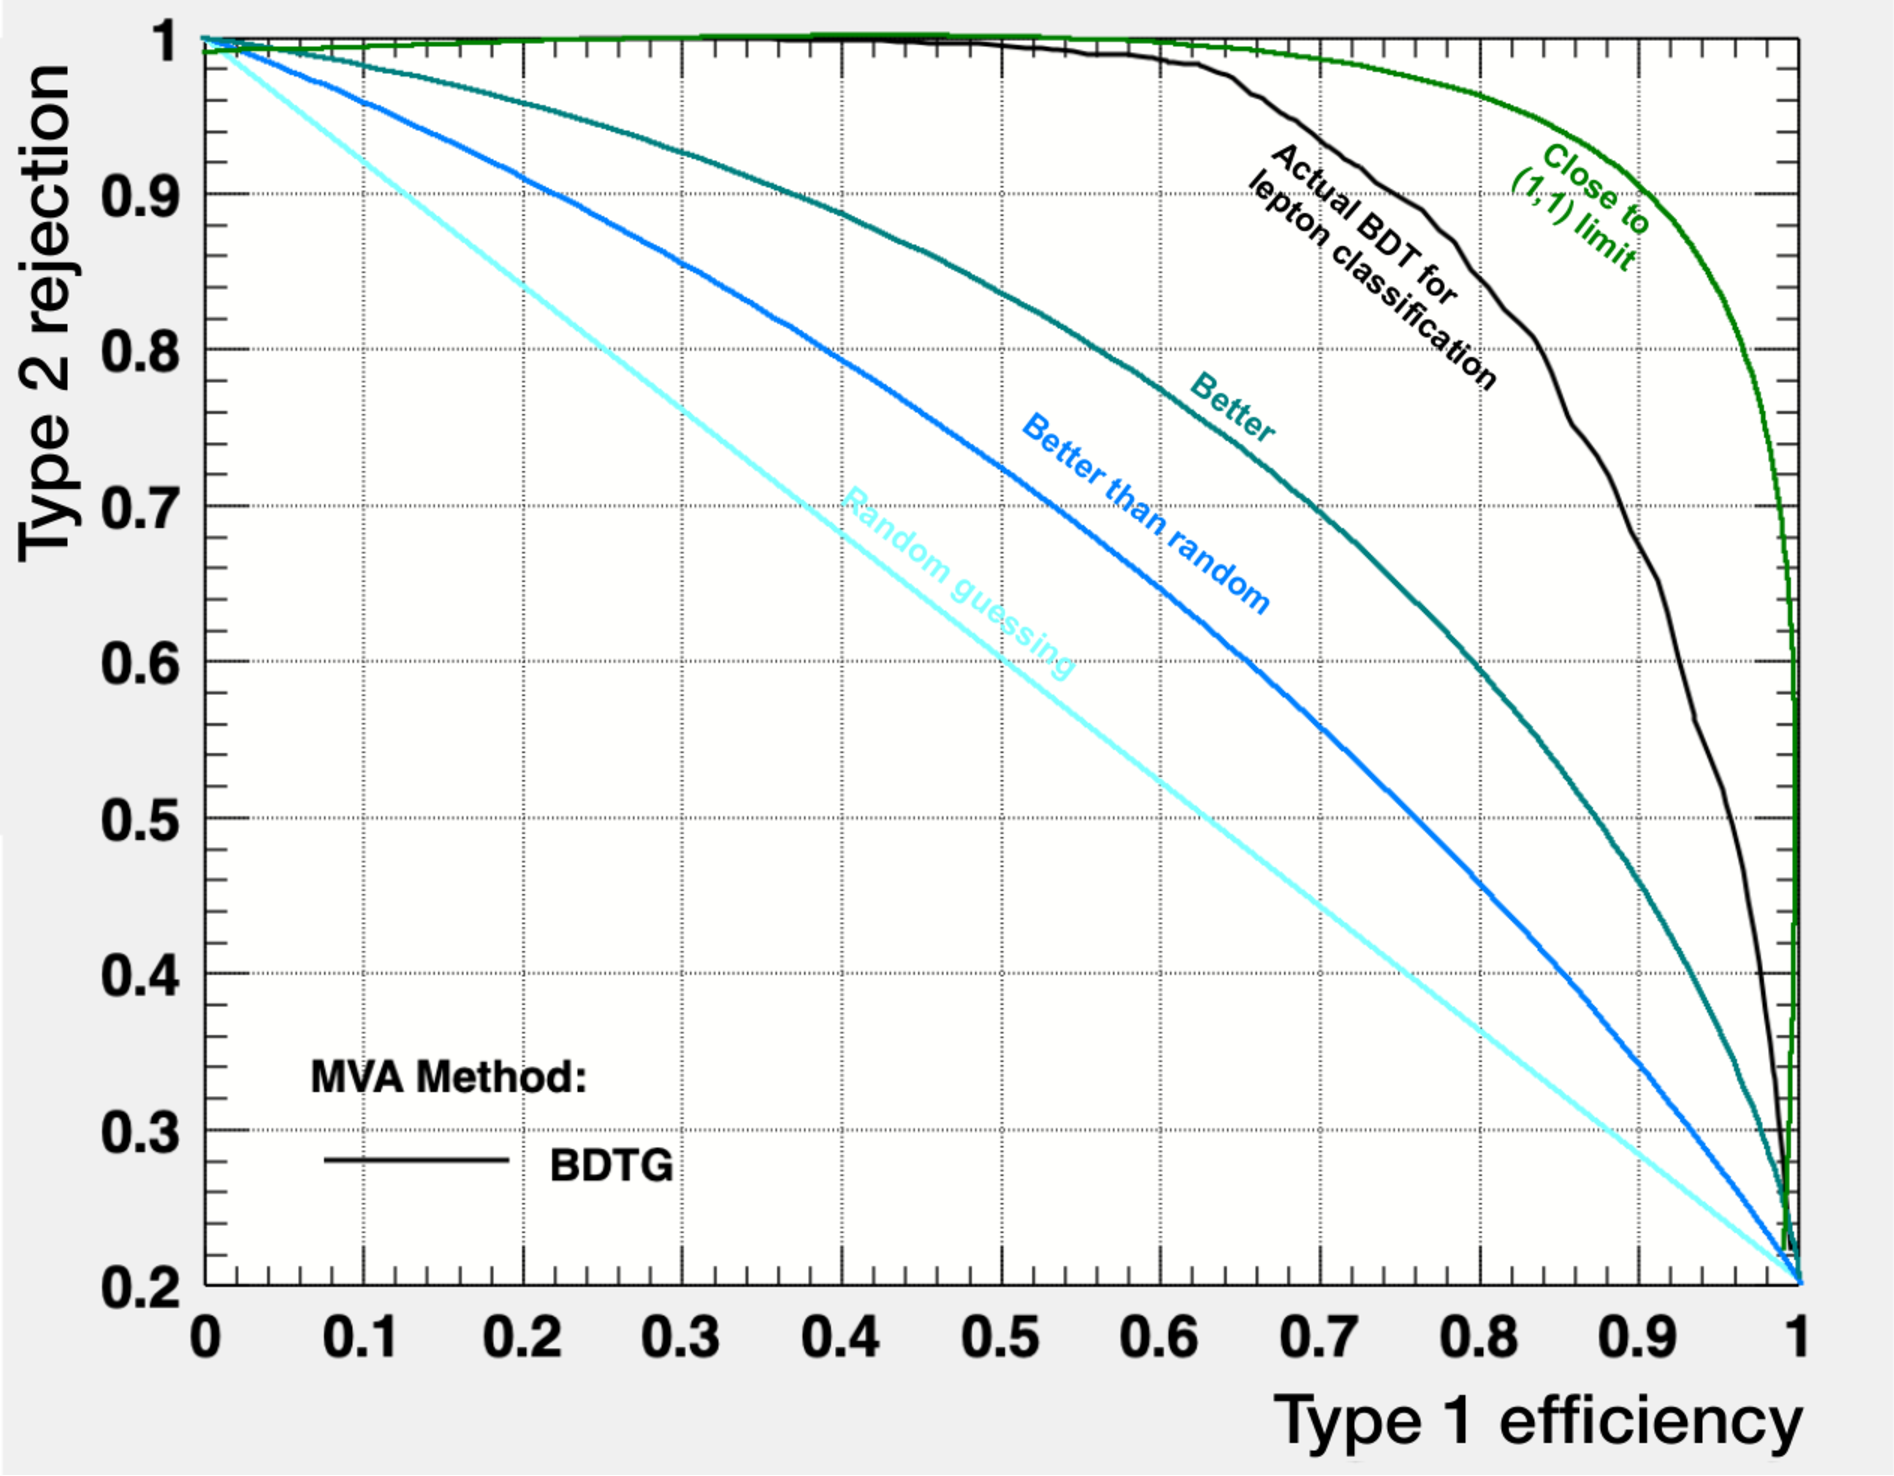
\includegraphics[width=.9\linewidth]{Appendices/BDT/precision-recall_pdf}
\caption{Precision-recall curves for different models. The one in black corresponds to the
model used for the light-lepton-origin assignment.}
\label{fig:Appendix:BDT:precision-recallCurve}
\end{figure}

For both the ROC and the precision-recall curves, the larger the area under the curve, the better.
Figure \ref{fig:Appendix:BDT:precision-recallCurve} shows that the optimal classifier is the one in 
which the curve in the precision-recall plot is close to (1,1).


% KS test
\paragraph{Kolmogorov-Smirnov test}\mbox{}\\
In statistics, the Kolmogorov-Smirnov (KS) test is a non-parametric method for comparing the equality 
of one-dimensional probability distributions. It is used to assess the similarity between 
a sample distribution and a reference probability distribution.

In the context of multivariate analysis, 
the distributions tested by the KS are the scores of the test and train. In other words, 
the test sample. If the score is close to zero, it may imply that the classifier is overtrained.
In the way it is implement in ROOT.TMVA, the ideal value is 0.5, although being above 0.01 is
considered enough.

%For any two random samples drawn from the same parent distibution, the
%KS test value would be distributed uniformly between 0 and 1. So ..
%so if you training weren't biased at all towards the training
%sample (note: this bias does not necessarily represent overtraining)
%then you'd for you test / training sample 'on average' expect a KS
%value of 0.5

Some sources argue that KS test requieres a large sample to be effective.
This  may explain the low values in for all folds in the ROOT.TMVA gradient
BDT used for the lepton-origin assignment.
% Source about sample size: https://root-forum.cern.ch/t/overtraining-test-obtained-from-tmva/32148
% Discussion; https://root-forum.cern.ch/t/kolmogorov-smirnov-test-values/32868

 
% Separation power
\paragraph{Separation power}\mbox{}\\
The separation power is a valuable metric for evaluating the performance 
of a variable or classifier in terms of its ability to distinguish the target process 
from other processes. The separation power $<S^{2}>$ of a classifier $y$ can 
be quantified using the integral:
\begin{equation}\label{eq:Appendix:BDT:SeparationPower}
	<S^{2}> = \frac{1}{2}\int \frac{(\hat{y}_{S} - \hat{y}_{B})^{2}}{\hat{y}_{S}+\hat{y}_{B}}dy \, ,
\end{equation}
where $\hat{y}_{S}$ and $\hat{y}_{B}$ are, respectively, the signal and background probability 
density functions of $y$.  The 1/2 factor is used to keep $<S^{2}>$ within the [$0, 1$] interval.
The separation is zero for identical signal and background shapes, and 
it is one for shapes with no overlap.
%\end{comment}



%%%%
% Hyper params
%%%%%
\subsection{Hyperparameters}
\label{fig:Appendix:BDT:Hyperparams}
Hyperparameters is the term used to refer to the specifications that control\footnote{The prefix ``hyper'' suggest that 
these parameters are on a higher level that modulates the training process.}
 the learning process of a ML algorithm. 

A ML model is defined by its model parameters, which are sat by the process of training. 
In order to reach some level of intelligence, the process of training a model involves 
selecting the optimal hyperparameters that the learning algorithm will use to learn the
ideal model parameters that accurately map the input variables ($\bm{x}$) to the labels ($y$).
The learning algorithm uses hyperparameters when learning, but these are not included 
in the resulting model. 

\subsubsection{XGBoost}
In XGBoost, the hyperparameters are classified in three categories: general, booster and task hyperparameters.
For the work developed in this thesis, the parameters related to the boosting of the trees are the ones
that have ben optimised. The process of finding the optimal set of hyperparameters for each model
is crucial to achieve success. 

\begin{itemize}
	\item General parameters: Refers to which booster its been used (typically a tree or linear model) are the number of
	parallel threads to be used (set to the maximum in our case). 
	\item Booster parameters: Control the performance of the selected booster. 
	For trees, the most relevant are: 
	\begin{itemize} %https://xgboost.readthedocs.io/en/stable/parameter.html#parameters-for-tree-booster
		\item \textbf{Learning rate}: 
		This tuning parameter in an optimisation algorithm 
		determines the step size at each iteration while moving toward a minimum of a loss function.
		Figure \ref{fig:Appendix:BDT:LearingRateTypes} shows the evolution per epoch for the loss function
		depending on the learning rate. This hyperparameter is also known as eta and ranges from 0 to 1.
			\begin{figure}
			\centering
  			\centering
  			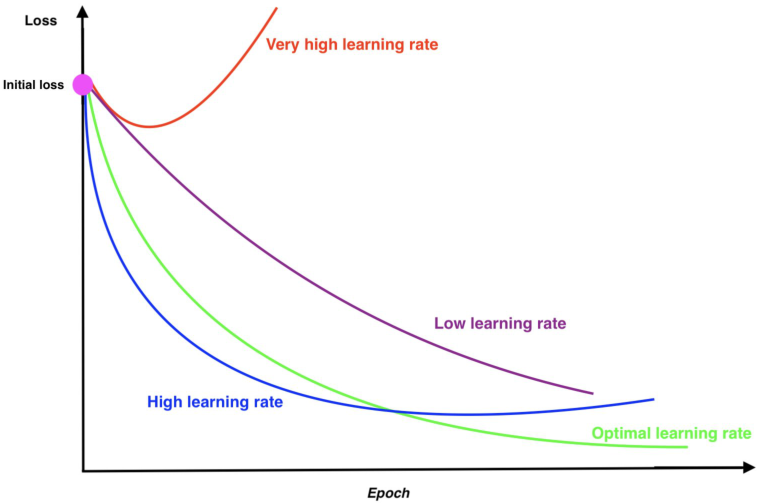
\includegraphics[width=.8\linewidth]{Appendices/BDT/LearningRateTypes}
			\caption{Different loss-function curves versus iteration.
			Learning rate is one of the most important hyperparameters to adjust well during the ML model training. 
			If it's high, it can cause the model to diverge. If it's too low it can slow down the training.}
			\label{fig:Appendix:BDT:LearingRateTypes}
		\end{figure}
		
		\item \textbf{Minimum split loss}: 
		Also known as gamma or Lagrangian multiplier. it is the 
		A node is split only when the resulting split gives a positive reduction in the loss function
		and the gamma gives the minimum loss reduction required to make a further partition
		 on a leaf node of the tree. Therefore, the higher the gamma, the more conservative the algorithm
		 will be. The minimum split loss rages from 0 to $\inf$. 
		 We are not optimising this parameter but using the default (not constrained). 
		 Nevertheless, values between 1 and 10 have been tested.
		%Reads on gamma hyperparam: https://medium.com/data-design/xgboost-hi-im-gamma-what-can-i-do-for-you-and-the-tuning-of-regularization-a42ea17e6ab6
		
		\item \textbf{Minimum child weight}: 
		It defines the minimum sum of weights of all observations required in a child.
		When the tree partition results in a leaf node with the sum of instance weight less than the value of 
		this hyperparameter, the tree stops partitioning. Higher min\_child\_weight prevent the model from learning
		too specific relation. So, this is done to prevent overfitting. This tuneable parameter ranges from 0 to $\inf$.
		
		\item \textbf{Maximum depth}: It refers to the number of splits in each tree, which controls the complexity 
		of the boosted ensamble. The maximum depth of a tree is an integer ranging from 1 to $\inf$ but is rare to have trees
		with depth higher than 10 since XGBoost aggressively consumes memory when training a deep tree.
		In our trees this hyperparameter is 4 or 5.
		
		\item \textbf{Scale of positive weight}: When the categories are imbalanced as it is the case for the signal
		and background categories in this analysis, the signal sample can be reweighted by this value to have a larger impact.
		The typical value to consider is the fraction between positive instances (signal) and negative instances (background). 
		When the BDT is targeting the identification of background processes this hyperparameter is also used although it
		does not take such extreme values.
		
		\item Maximum delta step: 
		
		%\item Subsample
		
		%\item Sampling method
		
		%\item Regularisation
		
		\item \textbf{Tree method}: It alludes to the tree construction algorithm used in XGBoost. Since the
		training of the BDTs takes place in ARTEMISA\footnote{ARTEMISA (ARTificial Environment for Machine
		learning and Innovation in Scientific Advanced computing) is a ML dedicated facility at IFIC. It is composed of 
		several Intel Xeon Platinum CPUs and Tesla Volta GPUs that help to find the optimal configuration for ML algorithms.} 
		facility \cite{ARTEMISA}, the method used here is the GPU implementation of the faster histogram 
		optimised approximate greedy algorithm.

		
		%\item \textbf{n_jobs}: We use -1
		
	\end{itemize}
	\item Learning task parameters: Decide on the learning scenario. Specify the learning task 
	and the corresponding learning objective.
\end{itemize}


\subsubsection{TMVA ROOT}
This section complementes the hyperparameter optimisation for the lepton-assignment BDT
that is described in Section \ref{sec:ChaptH:Sig:LepAsign:SS:BDT:hyperparameters}.
The ROOT.TMVA-based BDTs allow to configure the several training hyperparameters.
From those, the ones that have been explored are:
\begin{itemize}
	\item \textbf{Number of trees}: Number of trees in the forest. The more trees, the more complex the 
		model is and, hence, it can learn more. However, the complexity risk is that the BDT can learn 
		the specifics of the training sample, i.e., overtraining.
		% NTrees :: Int
		
	\item \textbf{Maximum tree depth}: Maximum depth allowed for each decision tree.
		The cell tree depth can be limited by using this option. When \texttt{MaxDepth} 
		is set to an integer value greater than zero, the created cell tree will not be deeper 
		than \texttt{MaxDepth}.  
		% MaxDepth :: Int
			
	\item \textbf{Minimum size for each node}: Minimum percentage of training events required in a leaf node.
	 	The default for classification: 5\%. 
		% MinNodeSize ::  Real
		
	\item \textbf{Number of cuts}: Control the number of cuts tested within 
		a variable in order to find the optimal cut value for a node splitting.
		% nCuts :: Int
		
	\item \textbf{Negative weight treatment}: Controls the approach for handling 
		events with negative weights during BDT training. The ROOT.TMVA library has options
		to include negative weights in the training by paring them with positively weighted
		and ``annihilating'' both events. This strategy has been tested but in the end, removing the negative
		events provided the best performance. 
		% NegWeightTreatment :: Str

		
		
	\item \textbf{BoostType}: Type of boosting algorithm. The options are
		% BoostType = Grad
		% source for boost types: https://fhernanb.github.io/libro_mod_pred/gradboost.html and TMVA manual
		\begin{itemize}
			\item \textbf{AdaBoost}: This is the most popular type of boosting algorithm and it
				uses an exponential loss function. Its name comes from ``adaptative boosting''.
				It consists on creating several weak trees, each of them adjusting what the previous one
				could not. This algorithm lacks robustness in presence of outliers or mislabelled data points,
				which can happen in the lepton-origin-assignment scenario.
			%\item RealAdaBoost
			%\item Bagging
			%\item AdaBoostR2: If this is used, the loss function has to be either
			%	Linear, Quadratic or Exponential.
			\item \textbf{Gradient boosting}: The ROOT.TMVA implementation of the gradient boost
				 uses the binomial log-likelihood loss function for classification. This algorithm attempts
				 to overcome the problem presented by AdaBoost regarding the outliers or mislabeled data.
				 %The gradient boos creates several trees in sequence and each predictor tree 
				% Grad
		\end{itemize}
		
	\item \textbf{Learning rate}: Also called shrinkage, it is the learning rate of the GradientBoost 
		algorithm. A small shrinkage demands the use of more trees in the BDT but 
 		can significantly improve the accuracy of the prediction.
		% Shrinkage :: Here I was using 0.1 and the ROC curves looked terrible. With 0.3 it got better.
		
		
	%\item \textbf{UseBaggedGrad}: %Only applicable for gradient boosting. 
	%	If used, only a random subsample of the events is used for creating the trees at each iteration.
		%UseBaggedGrad :: Bool
		
	\item \textbf{Use Bagged Boost}: If used, only a random subsample of the events 
		is used for creating the trees at each iteration. The ``bagged sample fraction''
		is the relative size of bagged sample to the original size of the data sample.
		%Only applicable for gradient boosting. At each iteration it uses 
		%UseBaggedBoost // BaggedSampleFraction.  ::  str/real
	
		
	 \item \textbf{BaggedSampleFraction}:
	 	% BaggedSampleFraction 
	
	\item \textbf{Pruning}: Method used for removing statistically insignificant
		branches For BDTs, rather than pruning it is suggested to 
		small trees (max. depth $\simeq 3$) and use ``NoPruning''.
		% PruneMethod
\end{itemize}


%%%%%%%%%%%%%%%%%%%%%
%             Extra plots and tables            %
%%%%%%%%%%%%%%%%%%%%%
\section{Additional plots and tables}

\begin{figure}[htbp!]
\centering
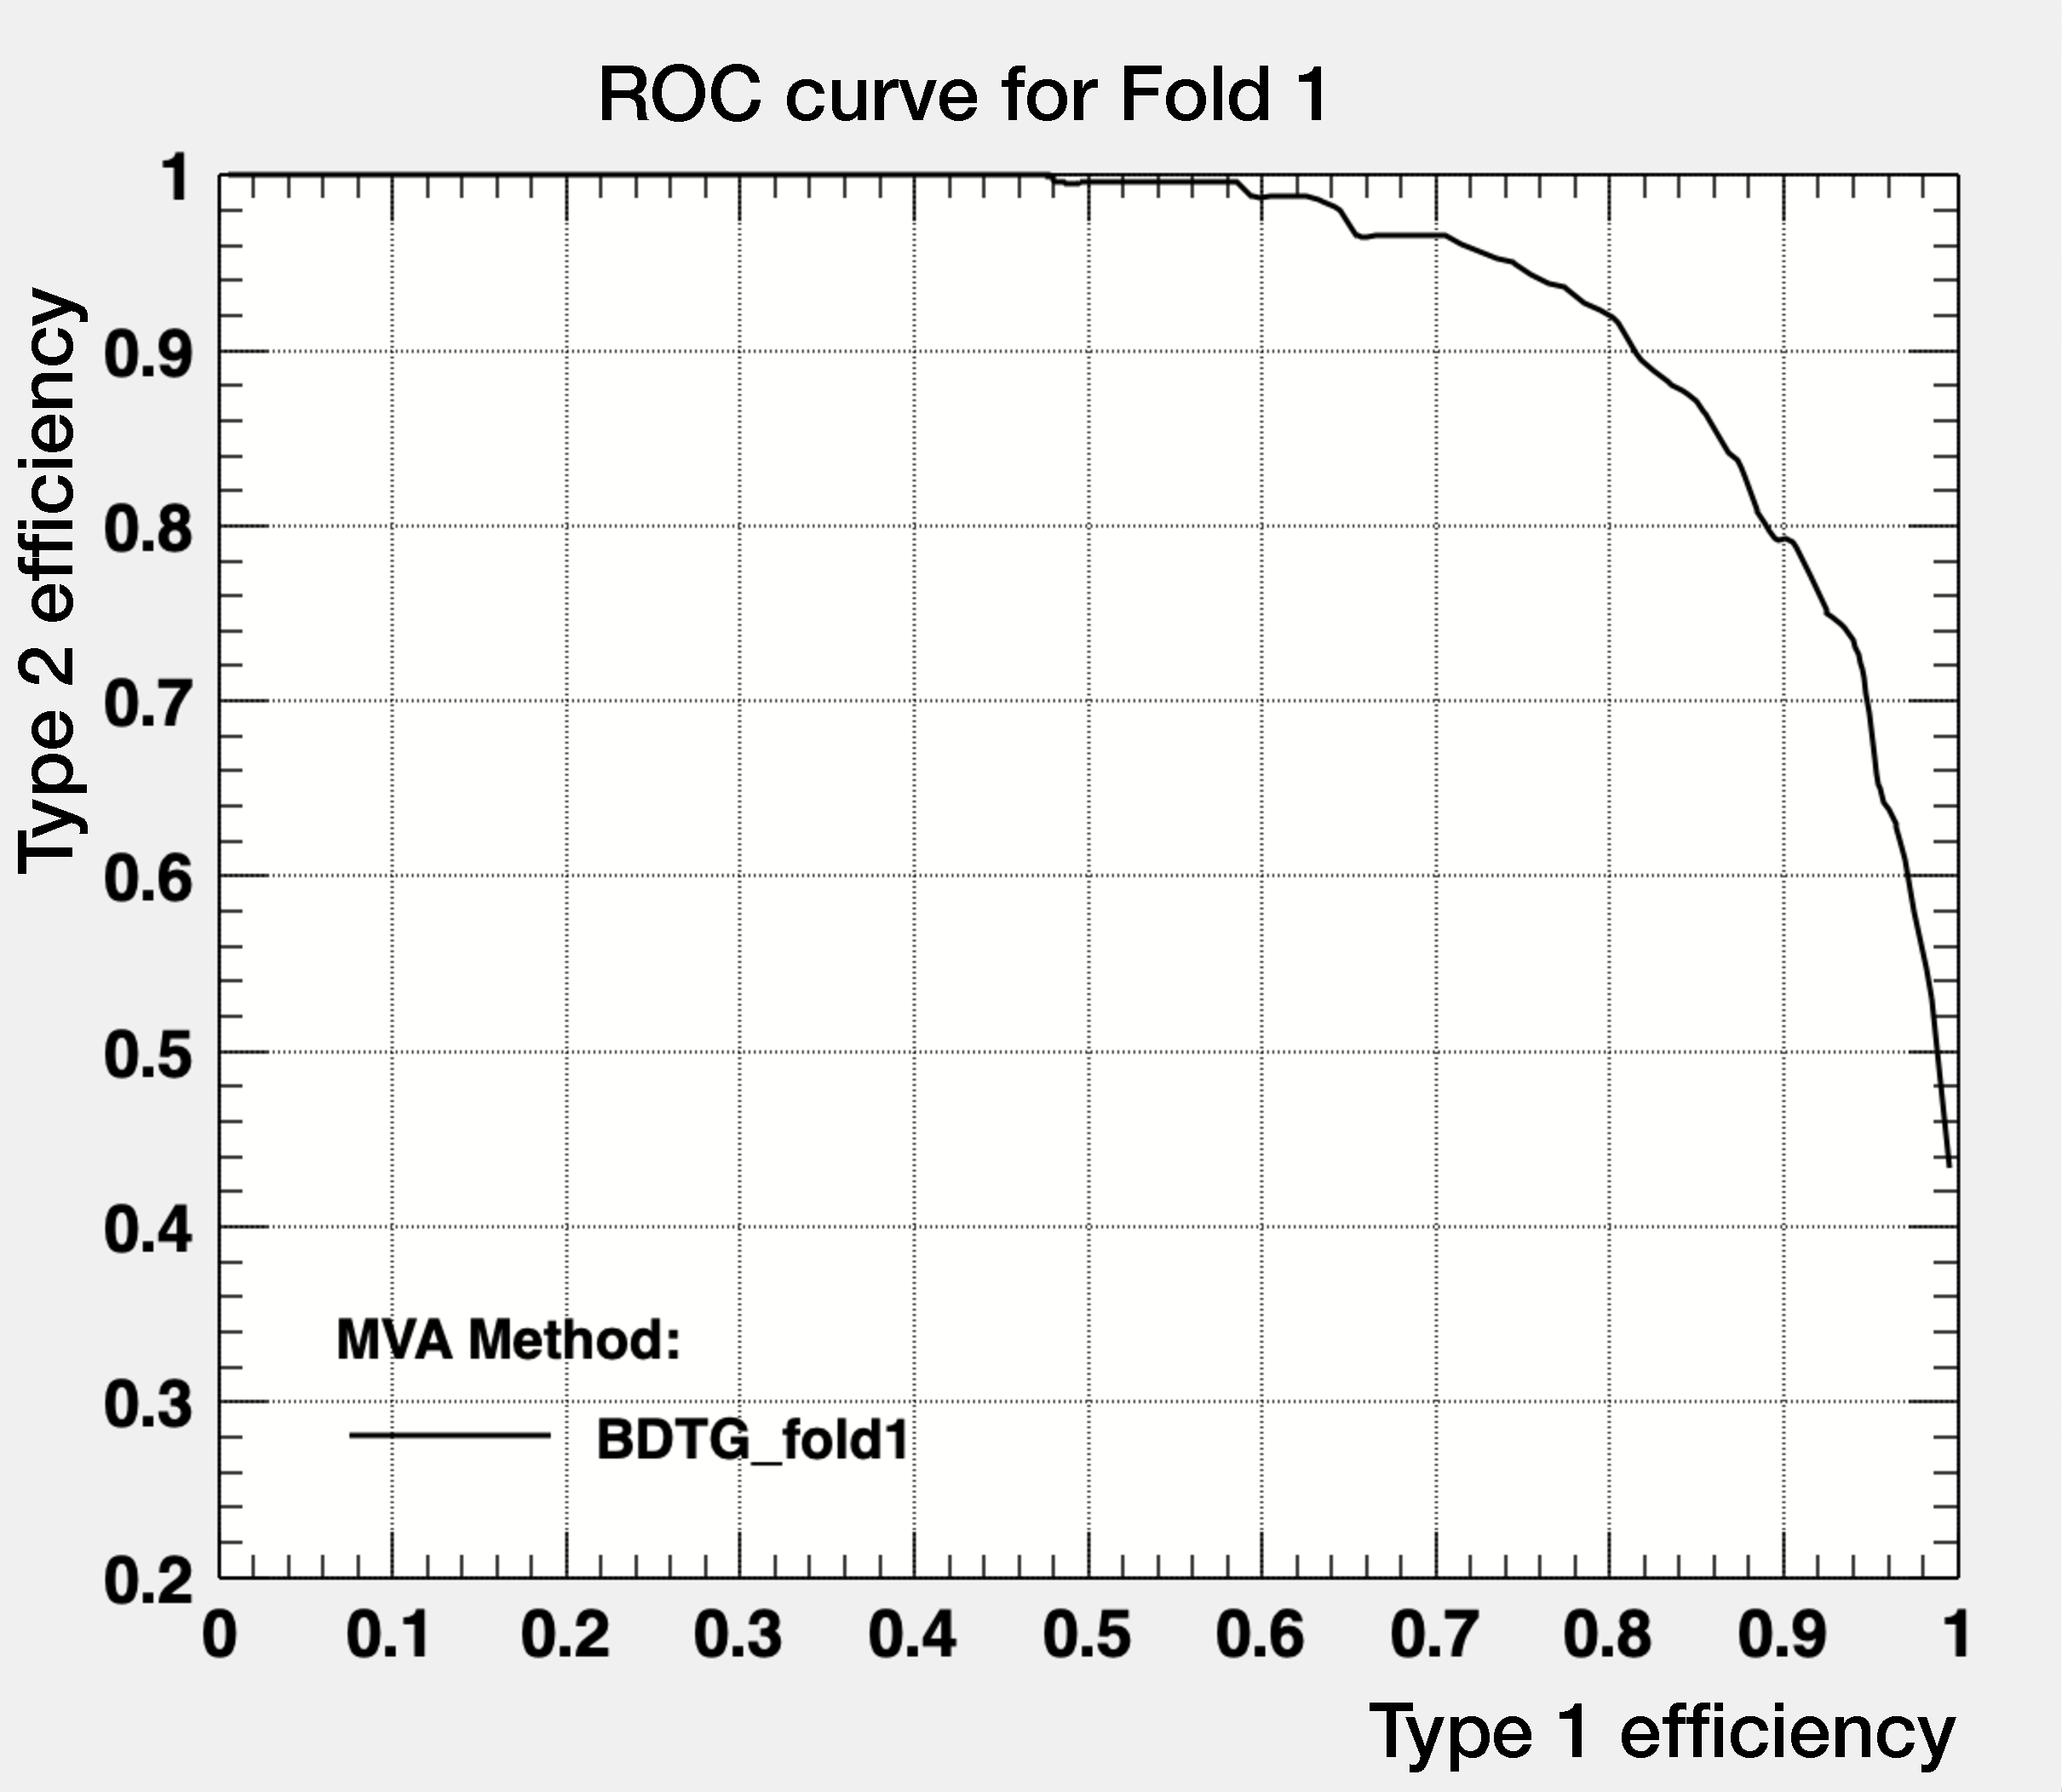
\includegraphics[width=.3\textwidth]{Chapter5_tHq/LeptAssociation/dileptau_ROC_Curve_Fold1}\quad
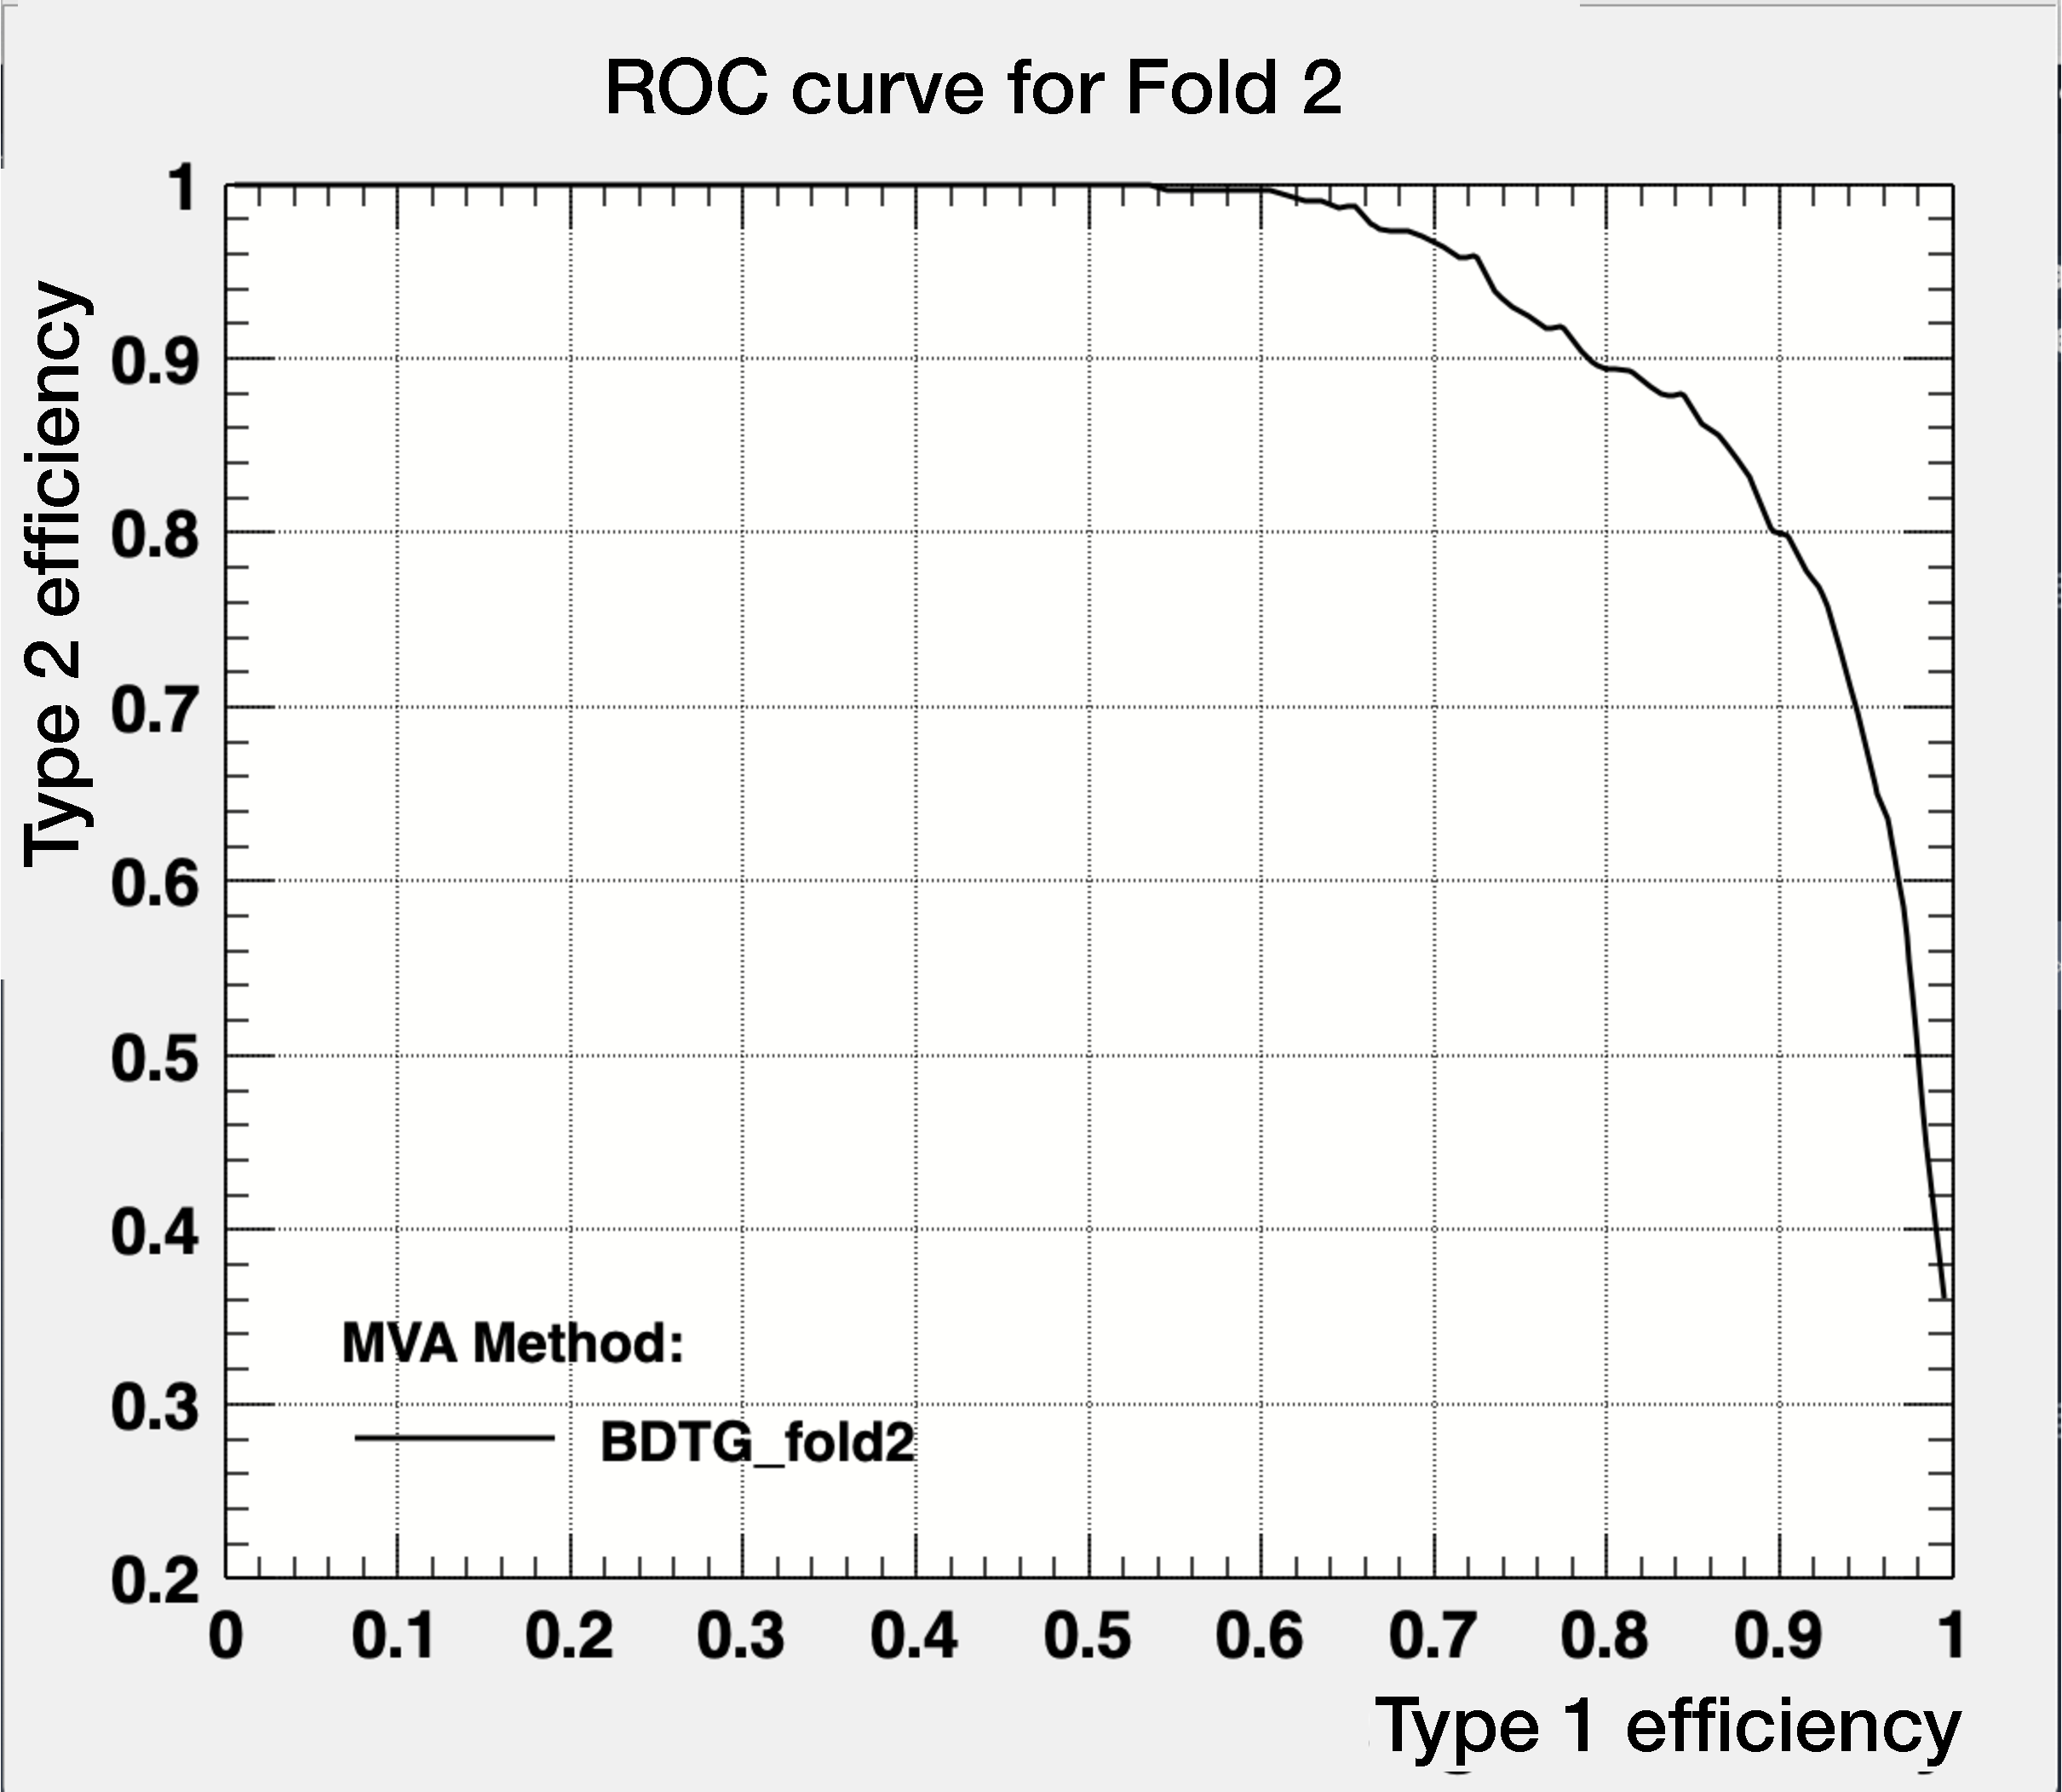
\includegraphics[width=.3\textwidth]{Chapter5_tHq/LeptAssociation/dileptau_ROC_Curve_Fold2}\quad
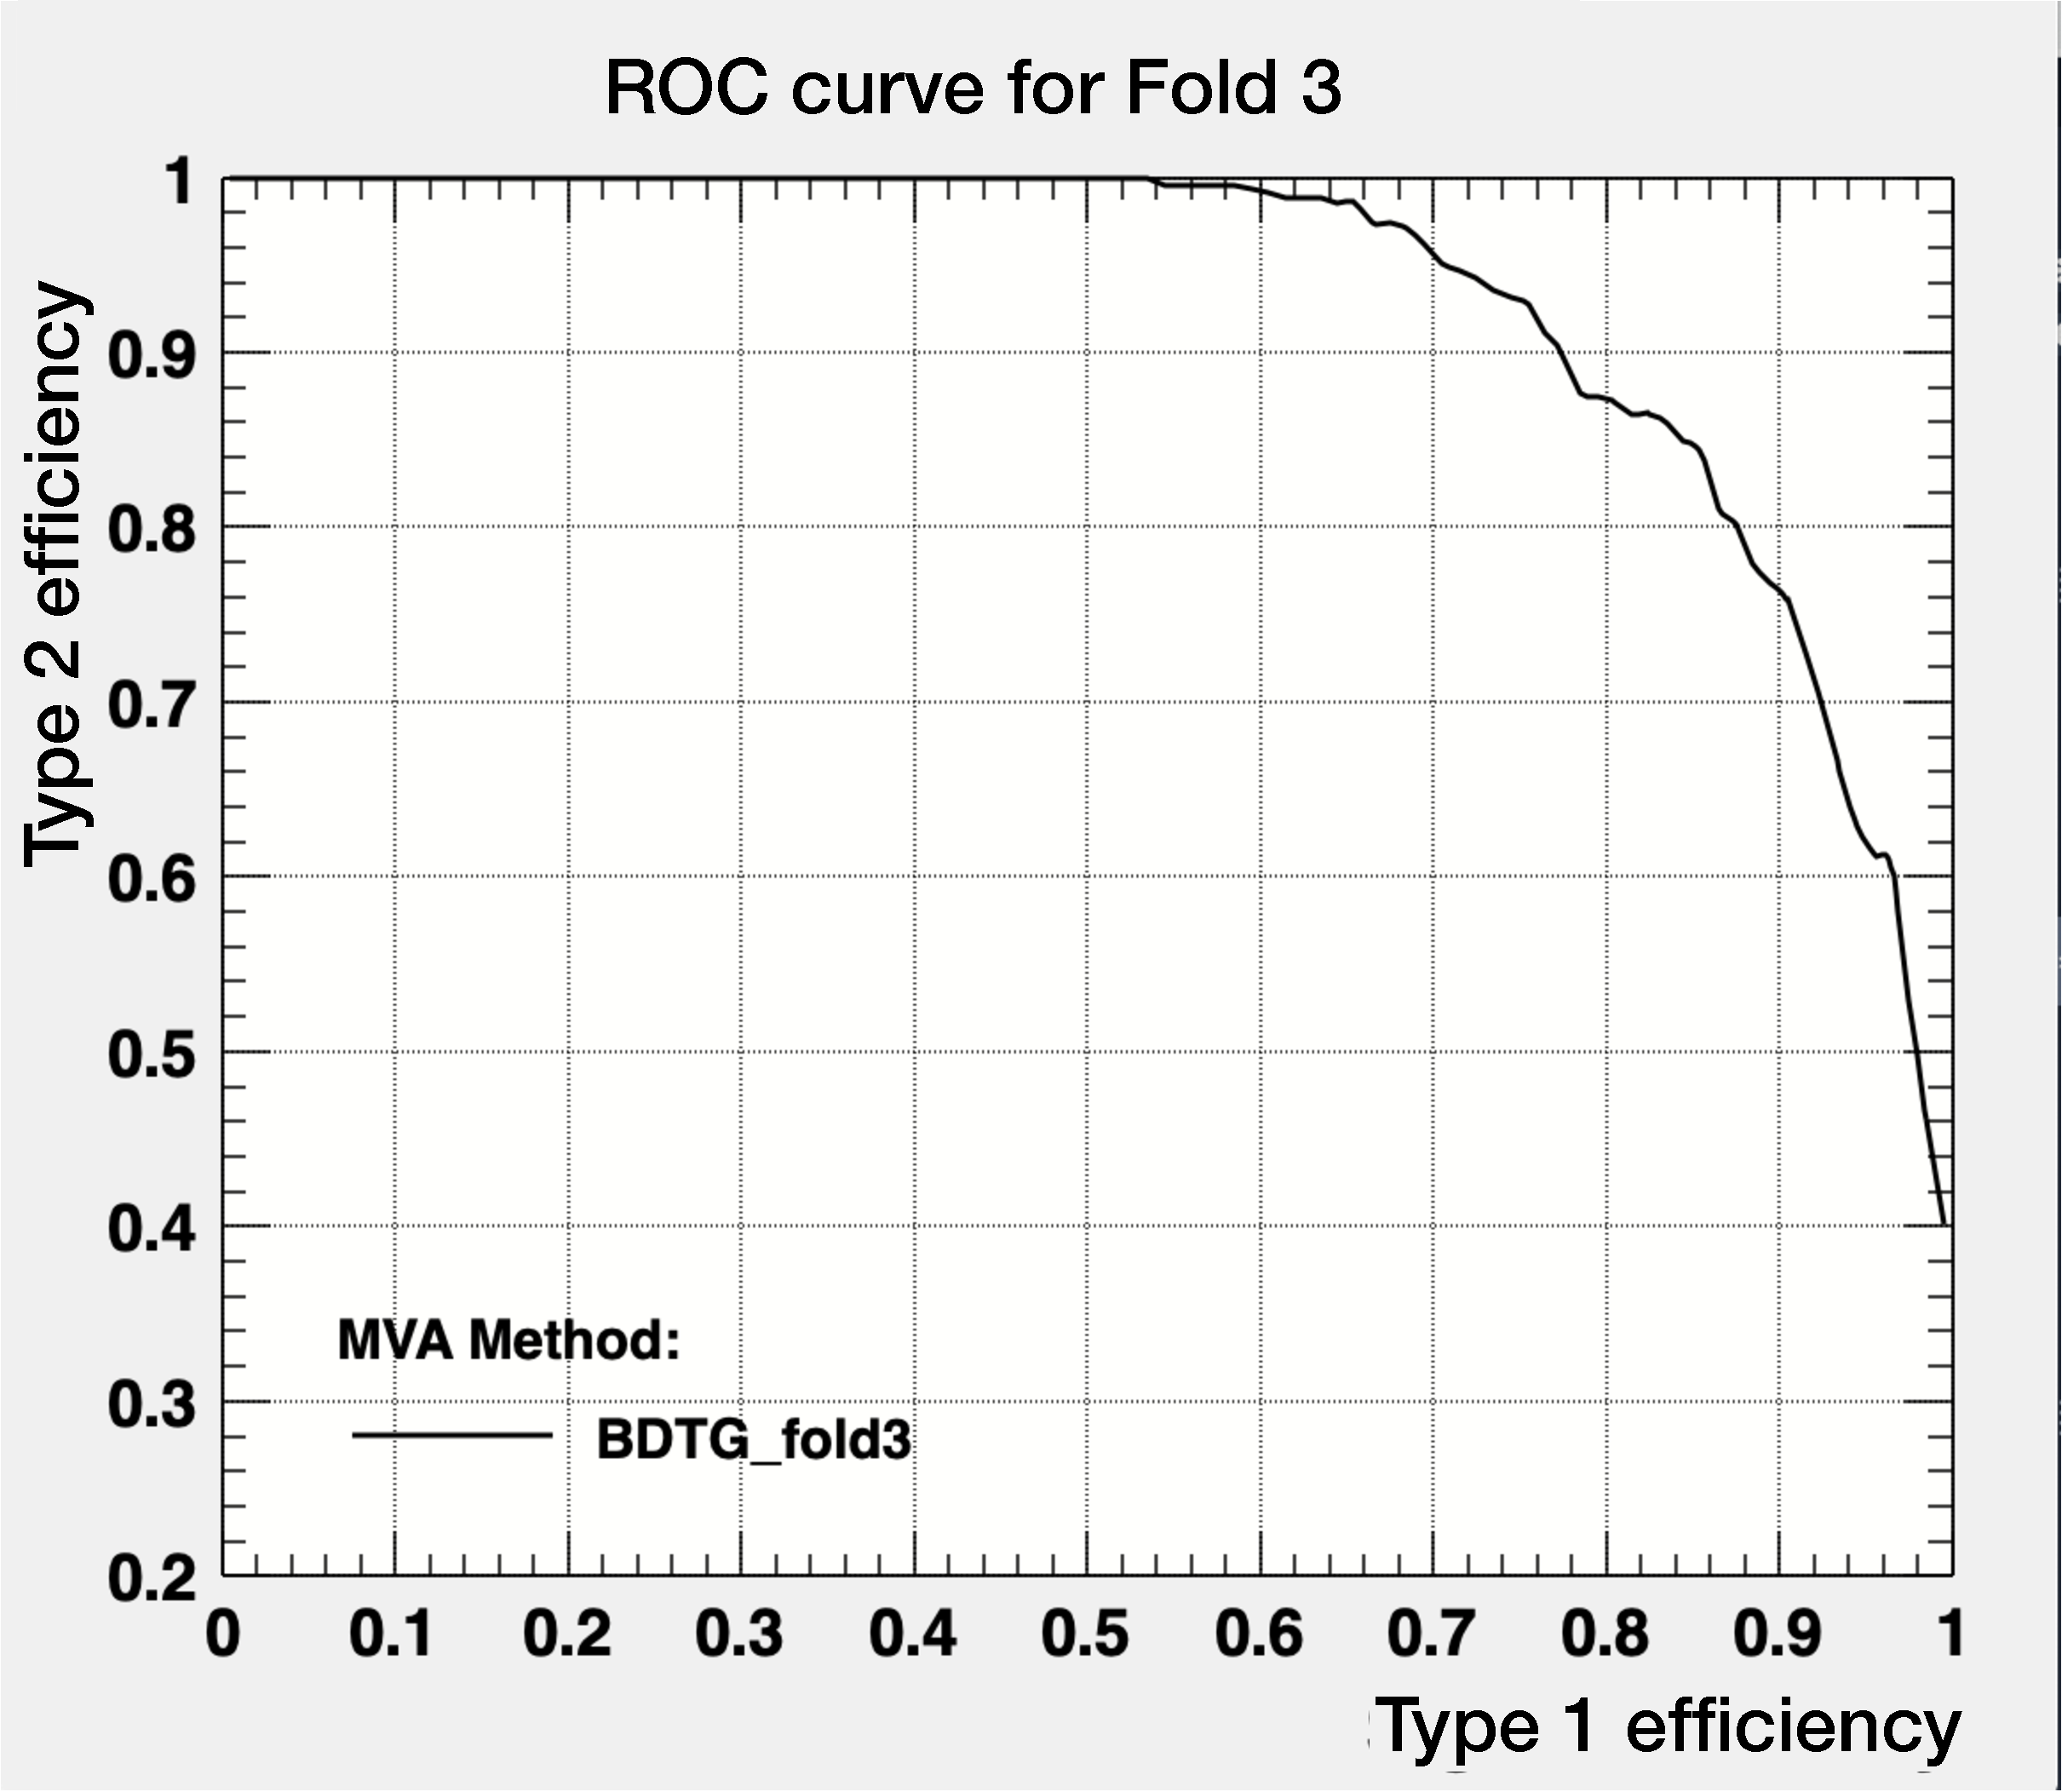
\includegraphics[width=.3\textwidth]{Chapter5_tHq/LeptAssociation/dileptau_ROC_Curve_Fold3}
\medskip
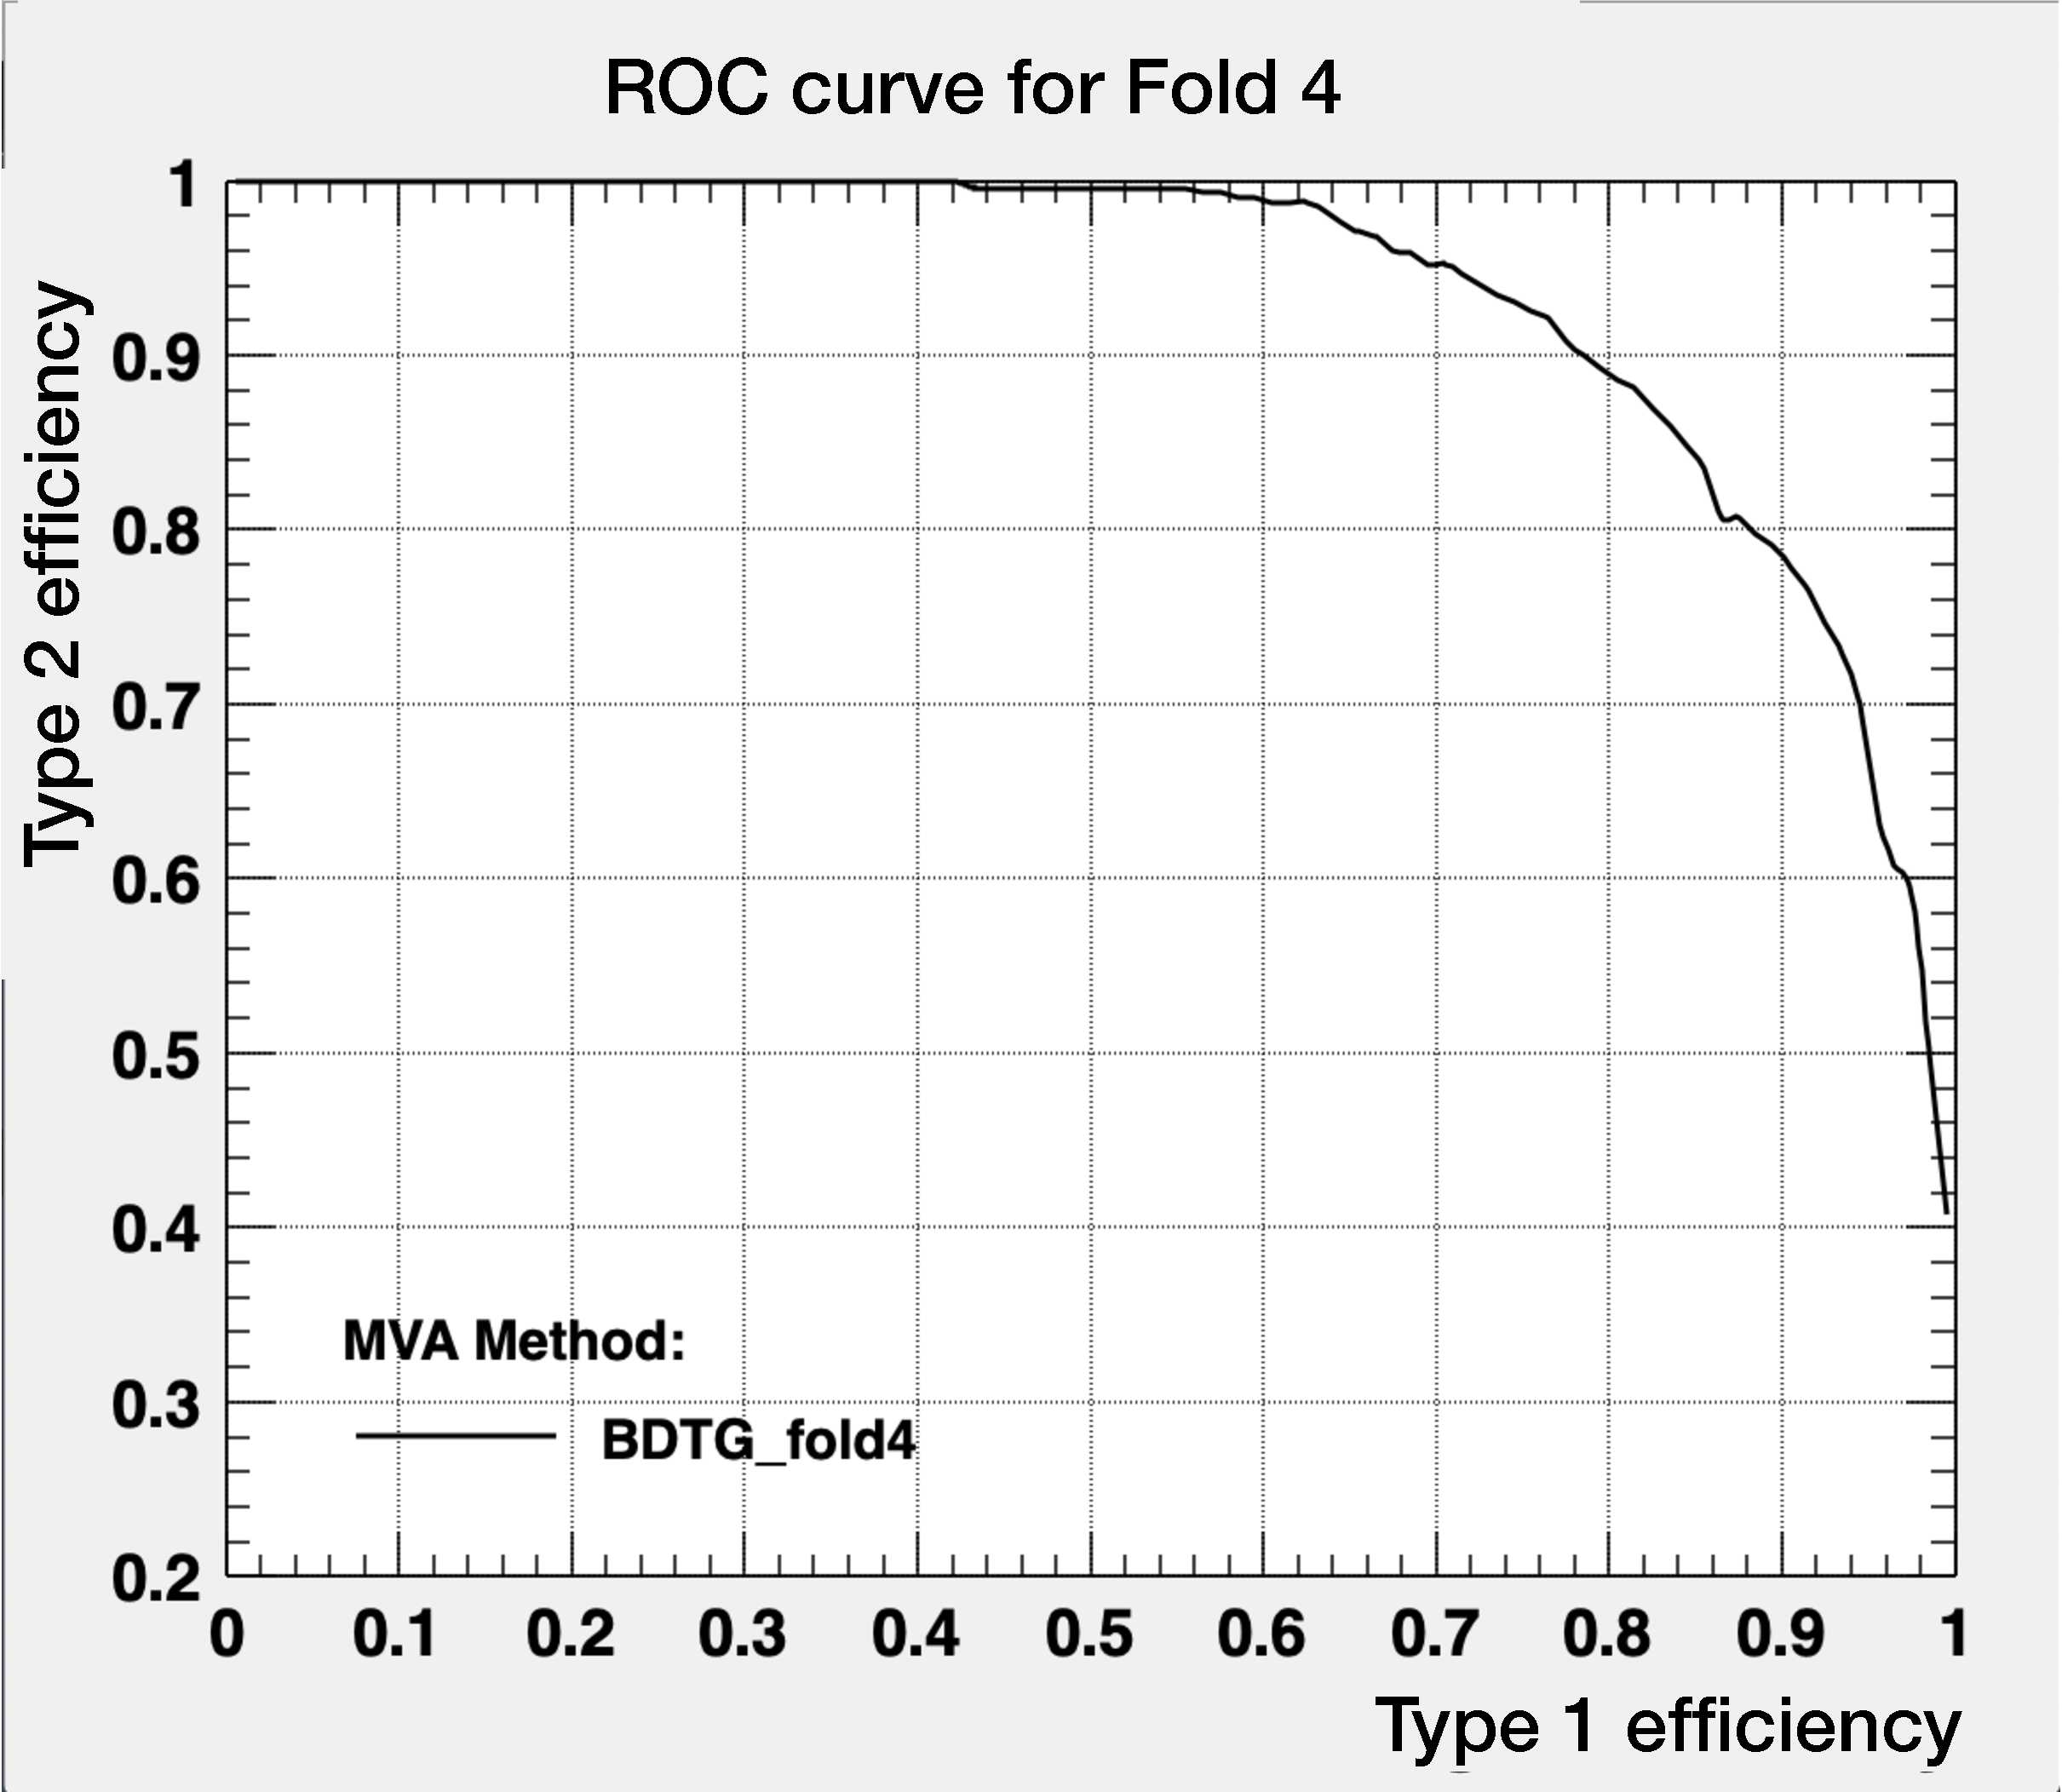
\includegraphics[width=.3\textwidth]{Chapter5_tHq/LeptAssociation/dileptau_ROC_Curve_Fold4}\quad
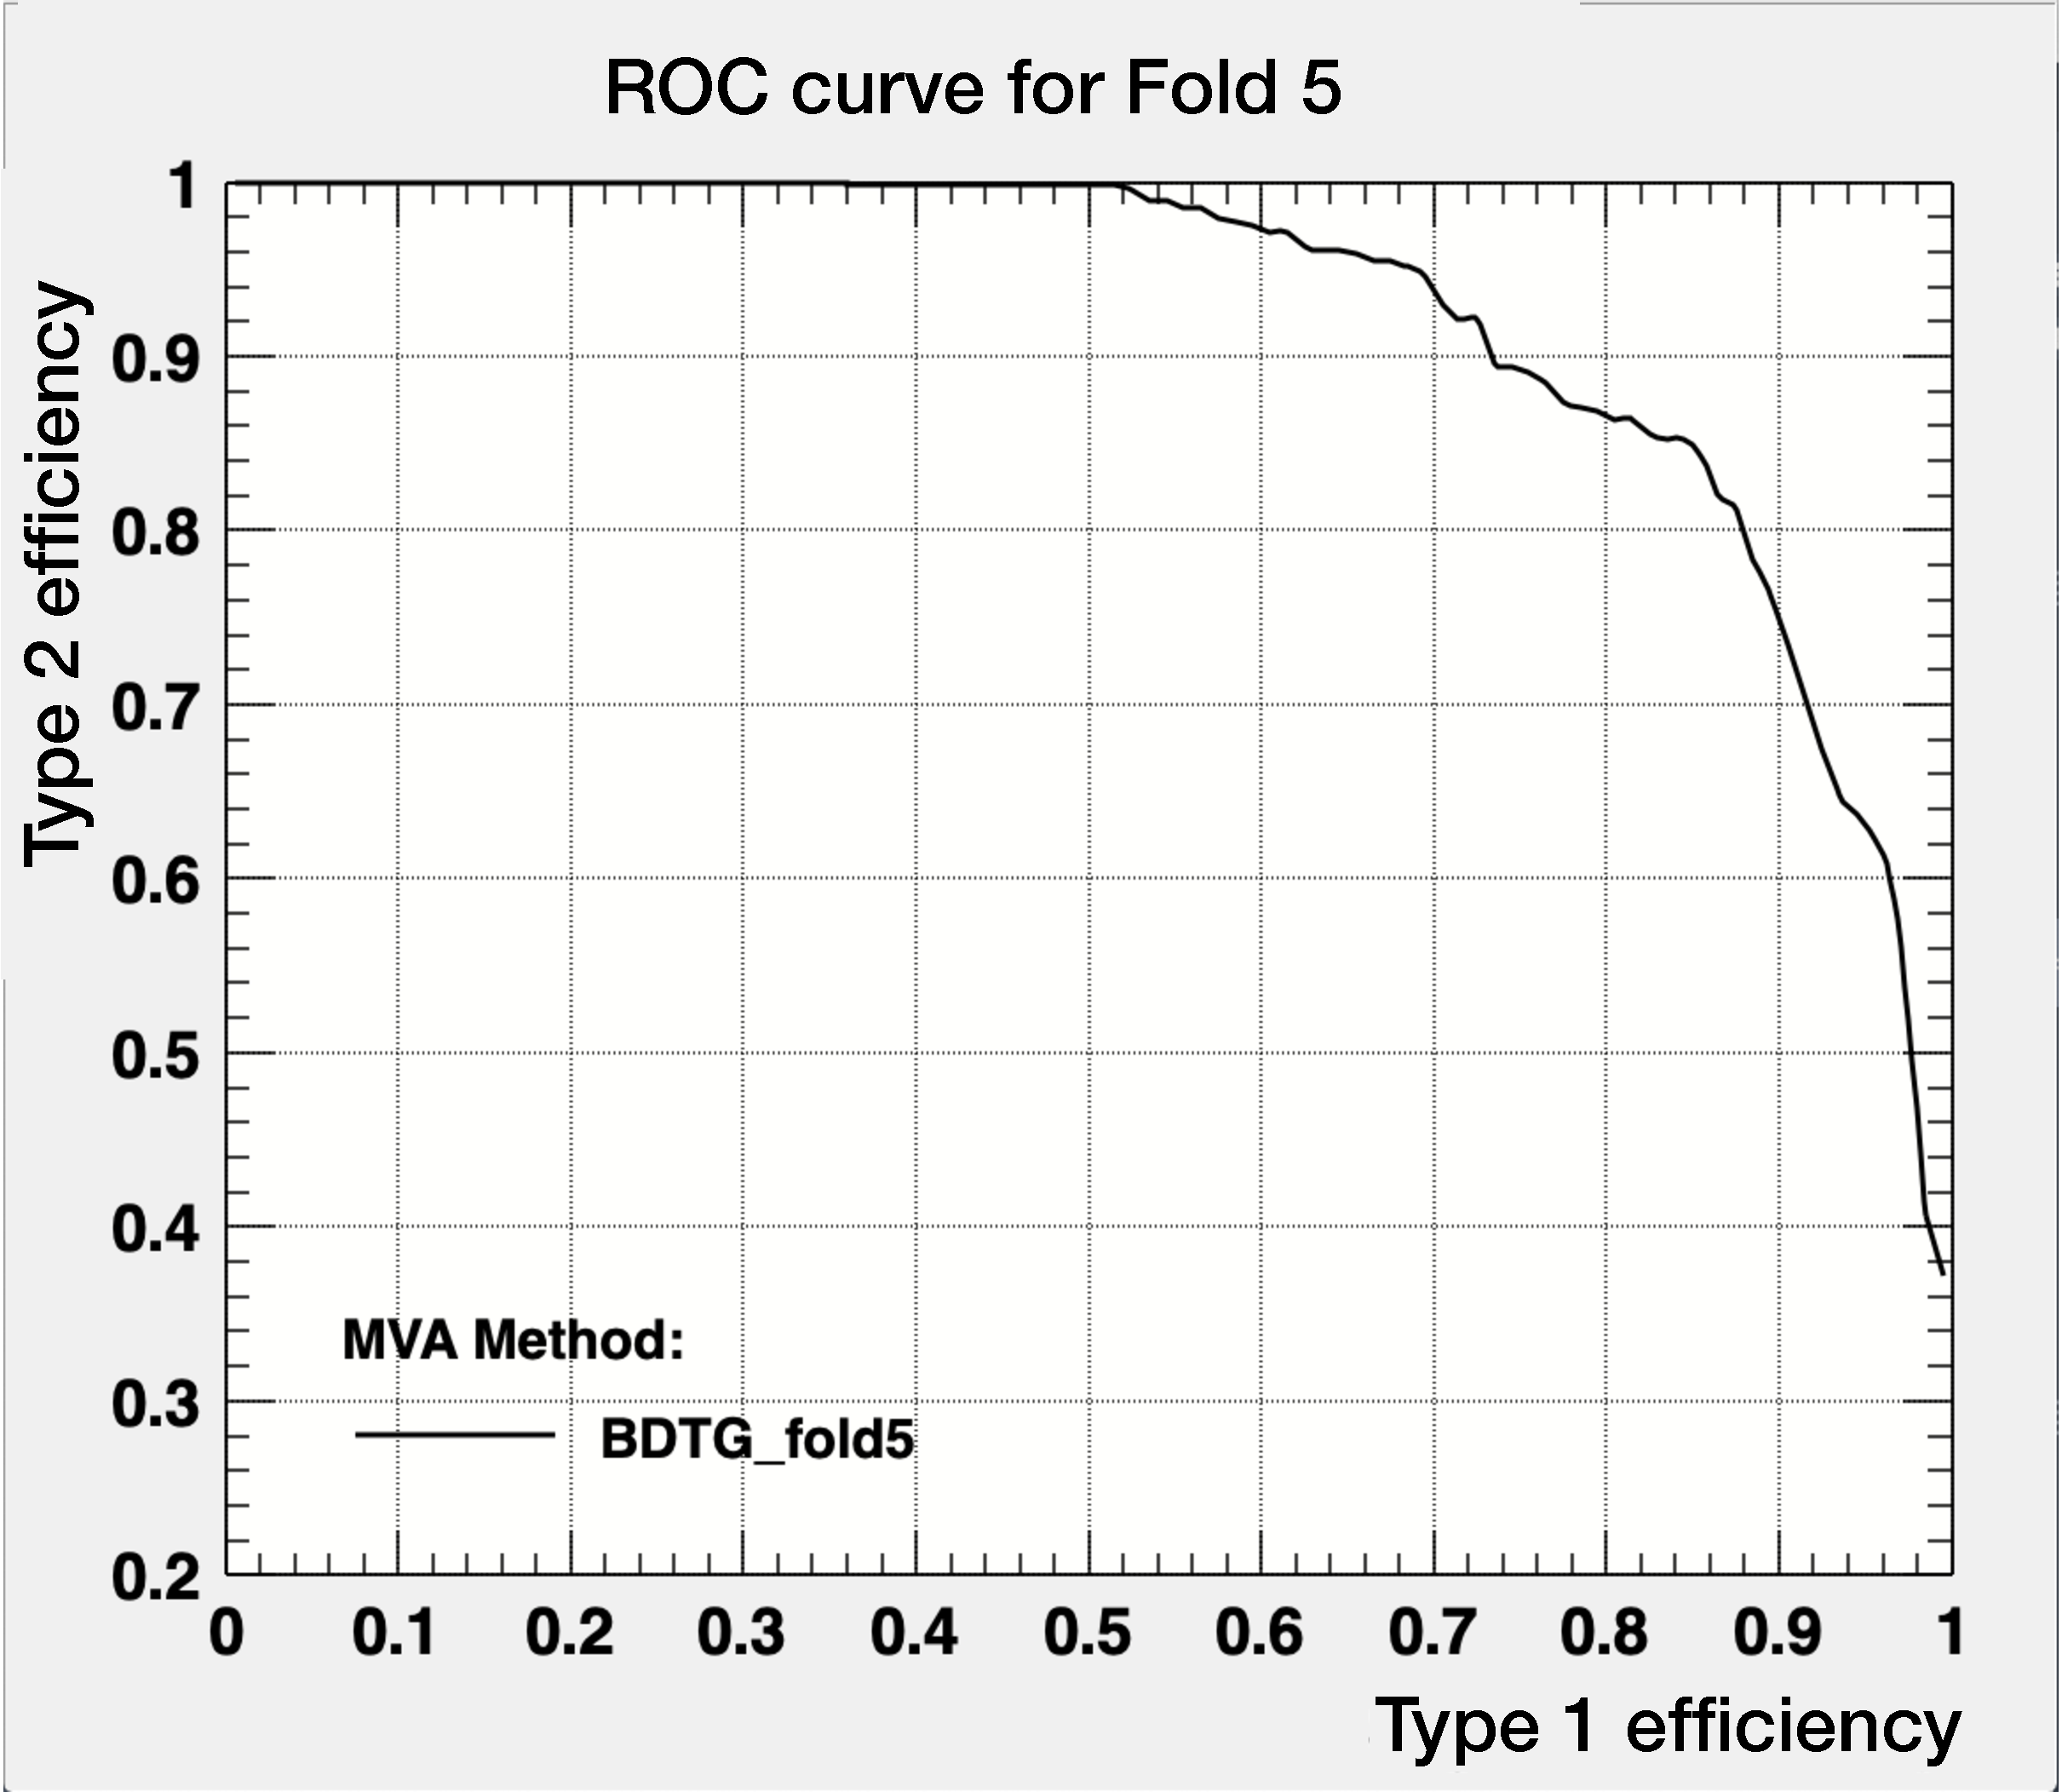
\includegraphics[width=.3\textwidth]{Chapter5_tHq/LeptAssociation/dileptau_ROC_Curve_Fold5}
\caption{ROC for the five different BDTs trained with k-folding.}
\label{fig:dileptau:Assignment_appendix:ROCs}
\end{figure}

\begin{table}[]
\centering
\resizebox{\textwidth}{!}{
\begin{tabular}{l|lllllllllllllllllllllllllll}
\toprule
BDT point         & -0.45 &    -0.4 &  -0.35 &  -0.33 & -0.32  & -0.315 & -0.31 & -0.395 & -0.3    & -0.29 & -0.28 & -0.27 & -0.25 & -0.2 & -0.15 & -0.1 & -0.05 & 0.0 & 0.05 & 0.1 & 0.15 & 0.2 & 0.25 & 0.3 & 0.35 & 0.4 & 0.45 \\ \midrule
Accuracy (\%)  & 88.12 & 88.03 & 87.97 & 88.23 & 88.33 & 88.39  & 88.36 & 88.32  & 88.15 & 87.85 & 87.89 & 87.99 & 87.84 & 87.62 & 87.47 & 86.87 & 86.84 & 86.57 & 86.57 & 86.6 & 86.22 & 86.81 & 86.56 & 86.15 & 86.12 & 85.22 & 84.77  \\
\bottomrule   
\end{tabular}}
\caption{Different thresholds for lepton association compared to its correspondent accuracy.}
\label{tab:dileptau:Assignment_appendix:Thereshold_large}
\end{table}



%%%%%%%%%%%%%%%%%%
%             Additional models           %
%%%%%%%%%%%%%%%%%%

\section{Alternative BDT-based Models}
In this section, we present some of the most relevant BDT-based models that were trained but not ultimately used in the final analysis of this PhD thesis. These models were developed as alternative approaches to tackle specific aspects of the analysis or to explore different signal and background processes. Although they were not included in the final analysis, they provide valuable insights and potential avenues for future research.


\subsection{Alternative Model for Lepton Assignment}

One of the BDT-based models developed during this study focused on improving the lepton assignment algorithm. The lepton assignment plays a crucial role in reconstructing the final state particles in many physics analyses. The alternative BDT model was trained to optimise the assignment of leptons in the event, taking into account their kinematic properties, isolation, and other relevant observables. Although this model showed promising performance in preliminary studies, it was not ultimately adopted in the final analysis due to the need for further validation and a thorough assessment of its impact on the analysis outcomes.

\subsection{BDT for \Zjets}
The production of Z bosons in association with jets (\Zjets) is an important background process for the \dilepOStau. To better discriminate between the \Zjets background and the signal process of interest, a dedicated BDT model was trained. 

However, further investigations revealed that the BDT model targeting \ttbar was achieving the same
same as the BDT for \Zjets, which was to separate these two proceses. Therefore, the decision was 
made to use only the BDT model for \ttbar, as it already effectively accounted for the separation from the \Zjets and \ttbar.



\subsection{BDT for tWH}
In order to comprehensively test the hypothesis $\yt = -1$, it is essential to consider not only the \tHq production process but also the \tWH process. To perform a combined fit where the entire \tH production is treated as a signal, it is important to have a BDT model that can effectively identify the \tWH process to fit it alongside \tHq.

The first practical approach consists on creating separate BDT models for each process rather than to  to have a single BDT model that targets both processes simultaneously. While it may seem intuitive to train a single BDT model targeting both processes, such an approach can be challenging due to the inherent differences between \tHq and \tWH events. Creating individual BDT models, one for \tHq and another for \tWH, allows for a more focused and optimised training process. Each model can be tailored to the specific characteristics and kinematic properties of its respective process, resulting in improved performance and discrimination power.







